% \iffalse meta-comment
%
% Package beamersubframe
% Copyright (c) 2011 Mike Kaufmann, all rights reserved
%
% This program is provided under the terms of the
% LaTeX Project Public License distributed from CTAN
% archives in directory macros/latex/base/lppl.txt.
%
% Author: Mike Kaufmann
%         m.km@gmx.de
% \fi
%% \CharacterTable
%%  {Upper-case    \A\B\C\D\E\F\G\H\I\J\K\L\M\N\O\P\Q\R\S\T\U\V\W\X\Y\Z
%%   Lower-case    \a\b\c\d\e\f\g\h\i\j\k\l\m\n\o\p\q\r\s\t\u\v\w\x\y\z
%%   Digits        \0\1\2\3\4\5\6\7\8\9
%%   Exclamation   \!     Double quote  \"     Hash (number) \#
%%   Dollar        \$     Percent       \%     Ampersand     \&
%%   Acute accent  \'     Left paren    \(     Right paren   \)
%%   Asterisk      \*     Plus          \+     Comma         \,
%%   Minus         \-     Point         \.     Solidus       \/
%%   Colon         \:     Semicolon     \;     Less than     \<
%%   Equals        \=     Greater than  \>     Question mark \?
%%   Commercial at \@     Left bracket  \[     Backslash     \\
%%   Right bracket \]     Circumflex    \^     Underscore    \_
%%   Grave accent  \`     Left brace    \{     Vertical bar  \|
%%   Right brace   \}     Tilde         \~}
%%
% \CheckSum{922}
%
% \iffalse meta-comment
%
%<*package>
%% 
\def\fileversion{0.2}
\def\filedate{2011/08/07}

%</package>
%
%<*driver>
\documentclass{ltxdoc}
\usepackage{hypdoc}
\usepackage{graphicx}
%\usepackage[pdfborder=0,colorlinks,linkcolor=blue]{hyperref}
\usepackage[all]{hypcap}
\setcounter{IndexColumns}{2}
\EnableCrossrefs
\CodelineIndex
%\RecordChanges
%\OnlyDescription
\makeatletter
% new, like ...Env... commands from doc.sty)
\let\PrintDescribeOpt\PrintDescribeEnv
\let\PrintOptName\PrintEnvName
\def\DescribeOpt{\leavevmode\@bsphack\begingroup\MakePrivateLetters
    \Describe@Opt}
\def\Describe@Opt#1{\endgroup
    \marginpar{\raggedleft\PrintDescribeOpt{#1}}%
    \SpecialOptIndex{#1}\@esphack\ignorespaces}
\def\SpecialOptIndex#1{\@bsphack
    \index{#1\actualchar{\protect\ttfamily#1}
           (option)\encapchar usage}%
    \index{options:\levelchar#1\actualchar{\protect\ttfamily#1}\encapchar
           usage}\@esphack}
% new (like \SpecialEnvIndex from hypdoc.sty)
\let\HDorg@SpecialOptIndex\SpecialOptIndex
\renewcommand*\SpecialOptIndex[1]{%
  \@bsphack
  \begingroup
    \HD@target
    \let\HDorg@encapchar\encapchar
    \edef\encapchar usage{%
      \HDorg@encapchar hdclindex{\the\c@HD@hypercount}{usage}%
    }%
    \HDorg@SpecialOptIndex{#1}%
  \endgroup
  \@esphack
}
% redefinition (from doc.sty)
\def\macro{\begingroup
   \catcode`\\12
   \MakePrivateLetters \m@cro@ \z@}
\def\environment{\begingroup
   \catcode`\\12
   \MakePrivateLetters \m@cro@ \@ne}
% new, environment 'option', like 'environment', but index entries with
% '(option)'
\def\option{\begingroup
   \catcode`\\12
   \MakePrivateLetters \m@cro@ \tw@}
% redefinition (from doc.sty)
\long\def\m@cro@#1#2{\endgroup \topsep\MacroTopsep \trivlist
   \edef\saved@macroname{\string#2}%
  \def\makelabel##1{\llap{##1}}%
  \if@inlabel
    \let\@tempa\@empty \count@\macro@cnt
    \loop \ifnum\count@>\z@
      \edef\@tempa{\@tempa\hbox{\strut}}\advance\count@\m@ne \repeat
    \edef\makelabel##1{\llap{\vtop to\baselineskip
                               {\@tempa\hbox{##1}\vss}}}%
    \advance \macro@cnt \@ne
  \else  \macro@cnt\@ne  \fi
  \edef\@tempa{\noexpand\item[%
     \ifcase #1%
       \noexpand\PrintMacroName
     \or
       \noexpand\PrintEnvName
     \or
       \noexpand\PrintOptName
     \fi
     {\string#2}]}%
 \@tempa
  \global\advance\c@CodelineNo\@ne
   \ifcase #1%
      \SpecialMainIndex{#2}\nobreak
      \DoNotIndex{#2}%
   \or
      \SpecialMainEnvIndex{#2}\nobreak
   \or
      \SpecialMainOptIndex{#2}\nobreak
   \fi
  \global\advance\c@CodelineNo\m@ne
  \ignorespaces}
% new
\let\endoption\endmacro
\def\SpecialMainOptIndex#1{\@bsphack\special@index{%
                                      #1\actualchar
                                      {\string\ttfamily\space#1}
                                         (option)%
                                      \encapchar main}%
    \special@index{options:\levelchar#1\actualchar{%
                   \string\ttfamily\space#1}\encapchar
           main}\@esphack}
\makeatother
\begin{document}
\DocInput{beamersubframe.dtx}
\end{document}
%</driver>
%
%<*package>
% \fi
%
% \DoNotIndex{\^}
% \DoNotIndex{\@auxout}
% \DoNotIndex{\@@end,\@empty}
% \DoNotIndex{\@gobble,\@gobbletwo}
% \DoNotIndex{\@ifclassloaded,\@ifnextchar,\@ifundefined}
% \DoNotIndex{\@makeother}
% \DoNotIndex{\@nameuse}
% \DoNotIndex{\@tempa,\@tempb,\@tempcnta,\@tempcntb}
% \DoNotIndex{\@writefile,\@nameuse}
% \DoNotIndex{\advance,\active,\addtocontents,\addtocounter}
% \DoNotIndex{\AtBeginDocument,\AtEndDocument}
% \DoNotIndex{\begin,\begingroup}
% \DoNotIndex{\beamer@endpageofdocument,\beamer@endpageofframe}
% \DoNotIndex{\beamer@endpageofpart,\beamer@endpageofsection}
% \DoNotIndex{\beamer@endpageofsubsection}
% \DoNotIndex{\beamer@frameendpage,\beamer@framepages,\beamer@framestartpage}
% \DoNotIndex{\beamer@startpageofpart,\beamer@startpageofsection}
% \DoNotIndex{\beamer@startpageofsubsection,\beamer@subsectionstartpage}
% \DoNotIndex{\beamer@partstartpage,\beamer@sectionstartpage}
% \DoNotIndex{\beamer@ifempty,\beamer@notesactions,\beamer@tempcount}
% \DoNotIndex{\c@framenumber,\c@page,\c@part}
% \DoNotIndex{\c@section,\c@subsection,\c@subsectionslide}
% \DoNotIndex{\catcode,\clearpage,\closeout,\csname}
% \DoNotIndex{\DeclareOption,\def,\do,\dospecials}
% \DoNotIndex{\edef,\else,\end,\endgroup,\endcsname,\endinput,\ExecuteOption}
% \DoNotIndex{\expandafter,\ExecuteOptions}
% \DoNotIndex{\fi,\filedate,\fileversion}
% \DoNotIndex{\gdef,\global}
% \DoNotIndex{\headcommand,\hyperlink}
% \DoNotIndex{\if@filesw}
% \DoNotIndex{\if,\ifcase,\ifcat,\ifdim,\ifnum,\ifx,\InputIfFileExists}
% \DoNotIndex{\immediate,\input}
% \DoNotIndex{\insertpartheadnumber,\insertsectionhead,\insertsubsectionhead}
% \DoNotIndex{\insertsectionheadnumber,\insertsubsectionheadnumber}
% \DoNotIndex{\jobname}
% \DoNotIndex{\let,\lastsubsection}
% \DoNotIndex{\MessageBreak}
% \DoNotIndex{\NeedsTeXFormat,\newcommand,\newcount,\newdimen,\newif}
% \DoNotIndex{\newenvironment,\newtoks,\newwrite,\noexpand}
% \DoNotIndex{\openout}
% \DoNotIndex{\PackageError,\PackageWarning,\PackageInfo}
% \DoNotIndex{\ProcessOptions,\ProvidesPackage}
% \DoNotIndex{\protect}
% \DoNotIndex{\relax,\RequirePackage}
% \DoNotIndex{\setcounter,\slideentry,\space,\string}
% \DoNotIndex{\the}
% \DoNotIndex{\verbatim@,\verbatim@line,\verbatim@processline}
% \DoNotIndex{\write}
% \DoNotIndex{\xdef,\z@}
%
% \changes{0.1}{2011/06/29}{initial release}
% \changes{0.2}{2011/08/07}{proper package, manual and documentation}
% \changes{0.2}{2011/08/07}{appendix tested}
% \changes{0.2}{2011/08/07}{fixed navigation bar}
% \changes{0.2}{2011/08/07}{total number of frames not counting appended frames}
% \changes{0.2}{2011/08/07}{new environment lastframe}
% \changes{0.2}{2011/08/07}{subslideentry}
% \changes{0.2}{2011/08/07}{inserttotalframenumberwithsub}
% \changes{0.2}{2011/08/07}{new option nominiframes}
% \changes{0.2}{2011/08/07}{defaults for bsf@sub...page... macros}
% \changes{0.2}{2011/08/07}{checking .sfp file}
%
% \newcommand{\BSF}{\textsf{BeamerSubFrame}}
%
% \title{The \BSF\ Package\\[1ex]
%     Reordering frames in the PDF file without reordering the source}
% \author{Mike Kaufmann\\\href{mailto:m.km@gmx.de}{\texttt{m.km@gmx.de}}}
% \date{\filedate\ (v\fileversion)}
% ^^A--------------------------------------------------------------------------
% \maketitle
% \begin{abstract}
% The \BSF\ package provides a method to reorder frames in the
% PDF file without reordering the source. Mainly, it is meant to embed or
% append frames with details on some subject.
% \end{abstract}
%
% \tableofcontents
%
% ^^A--------------------------------------------------------------------------
% \section{Introduction}
% \subsection{Why this Package}
% Of course, usually a presentation is prepared for one occasion.
% But sometimes a presentation is used more then once, and the audience
% and/or the available time differs.
%
% For me, there are two kinds of audience. The first group are the
% sales people, who for the most part only want to know the features
% of a new product I developed. And the second group are the technicians,
% who want to know everything.
%
% So basically, on one time I have to give a presentation in half an hour,
% covering only the basics. But there might be questions, where I need to
% show some details. In this case it's nice to have the necessary frames.
% And an another time, I have to give a presentation in one hour, covering
% also the details.
%
% In both cases, it would be nice to have a presentation, where normally
% only the cursor keys are needed for navigation, and without the necessity
% of clicking on links.
%
% With Beamer, one would have to create two presentation. One with the
% frames containing details at the end, and another one with the details
% between the other frames.
%
% Now here the \BSF\ package comes in handy. After some changes to the source
% of the presentation with the details embedded, both version can be compiled
% out of the same source. To select the version, only one option must be
% changed.
%
% ^^A---------------------------------------------
% \subsection{A Warning}
% This package is in an early state of development (it's version
% \fileversion). It is already useful, but there are some restrictions (see
% \autoref{sec:restrictions}). And although it's not planned, the user
% interface may change in the future.
%
% ^^A---------------------------------------------
% \subsection{Feeback and Testing}
% Because this package is very new and still under development, any feedback
% is appreciated. A good location for a discussion would be the newsgroup
% \texttt{comp.text.tex} (or \texttt{de.comp.text.tex}).
%
% And since Beamer offers a lot of features and it is hard to test the
% \BSF\ package with all of them, it would be nice, if some people would
% do some additional testing and/or provide some presentation for testing.
%
% ^^A---------------------------------------------
% \subsection{Dependencies}
% The \BSF\ package can only be used with the Beamer class (article mode
% is not supported yet).
%
% Additionally, it needs the |verbatim| package.
%
% ^^A---------------------------------------------
% \subsection{Legal Stuff}
% This program is provided under the terms of the
% \LaTeX\ Project Public License distributed from CTAN
% archives in directory macros/latex/base/lppl.txt.
% 
% ^^A--------------------------------------------------------------------------
% \section{Using the Packages}
% \subsection{Package Options}
% The \BSF\ package has three options.
% 
% \DescribeOpt{embed}
% The option |embed| is used to put frames with details between the other
% frames.
%
% \DescribeOpt{append}
% The option |append| is used to remove the frames with details from the other
% frames and append them at the end of the PDF file.
%
% If none of these two options is given, |embed| is used as default. Both
% options are mutually exclusive. If both are given, the last one wins.
%
% \DescribeOpt{nominiframes}
% In themes with miniframes, there are also frame symbols for appended frames
% with details by default. If the option |nominiframes| is given, these frame
% symbols will disappear. This option has only an effect, if the |append| option
% is given too.
%
% ^^A---------------------------------------------
% \subsection{The \texttt{subframe} Environment}
% \DescribeEnv{subframe}
% For frames which should be embedded or appended contitionally (i.e.\ frames
% with details), the |subframe| environment must be used instead of the |frame|
% environment. Basically, it works the same way as the |frame| environment,
% i.e.\ it has the same options and arguments.
%
% For typesetting, the |frame| environment is used internally. In embed mode
% (i.e.\ the |embed| option is given) it inserts the option |environment=subframe|
% to enable the use of verbatim material in the frames. In append mode the contents
% of the frame is written to a file. Before the contents, |\begin{frame}|, with
% all arguments of the |subframe| environment appended, is inserted. And after
% the contents |\end{frame}| is inserted.
%
% For copying the contents, the |verbatim| package is used. So in append mode
% the |subframe| environment is treated as a |verbatim|
% environment,\footnote{Because of this, the phrase \texttt{\bslash
% end\{subframe\}} cannot be used in a \texttt{subframe} environment.} but
% without typesetting anything.
%
% There should be no parts, sections, or subsections only containing subframes,
% because in append mode, they would have no contents. Since it is not the
% intention of the \BSF\ package, to move parts, sections, or subsections, this
% was not even tested.
%
% ^^A---------------------------------------------
% \subsection{Appending Frames}
% \DescribeMacro\appendsubframes
% To append the subframes, the macro |\appendsubframes| must be called before
% |\end{document}|. In embed mode, the command simply does nothing. In append
% mode it inputs the file written by the |subframe| environments.
%
% The command is only allowed once and it can only appear right before
% |\end{document}|.\footnote{Both restrictions are not tested by the package yet.}
% Disregarding this may lead to some strange errors.
%
% The command can be omitted to remove the subframes from the PDF file in append
% mode. But links to them will then produce warnigs and will lead somewhere else.
% In themes with miniframes, the links of the miniframe symbols for subframes
% will lead to page 1.
%
% ^^A---------------------------------------------
% \subsection{Conditional Execution}
% \DescribeMacro\ifappend
% To execute some macros or insert some text according to the mode of the
% \BSF\ package, the marco |\ifappend| can be used. It has two arguments.
%
% \vspace{1ex}
% |\ifappend{|\meta{material for append mode}|}{|\meta{material for embed mode}|}|
%
% \vspace{1ex}
% \noindent
% The first argument is inserted only in append mode and the second one only in
% embed mode.
%
% The macro is intended for conditional links in frames and subframes. It can
% be used in own macros. To do something only in one mode, the argument for the
% other mode can be left empty.
%
% ^^A---------------------------------------------
% \subsection{The \texttt{lastframe} Environment}
% \DescribeEnv{lastframe}
% Normally, a presentation has a last frame, containing something like ``Thanks
% for listening'' (at least I learned it this way). But using a |frame|
% environmet, the navigation (sidebar, miniframes, and so on) appears as if the
% frame belongs to the last (sub)section.
%
% Using the |lastframe| environment, the navigation has the same appearance as
% on the title frame.
%
% It has the same options and arguments as the |frame| environment, which is
% used internally with all given arguments.. To enable the use of verbatim
% contents, it additionally inserts the option |environment=lastframe|.
%
% The |lastframe| environment must be used only for the last frame (before the
% |\appendsubframes| command), because it sets the counters for parts, sections,
% and subsections to 0. So after a ``lastframe'', sectioning will not work
% properly anymore.
%
% ^^A---------------------------------------------
% \subsection{Inserts}
% \DescribeMacro\inserttotalframenumber
% Beamers |\inserttotalframenumber| was changed. In append mode it now contains
% the number of frames without the subframes. In embed mode it contains the
% number of frames as usual.
%
% \DescribeMacro\inserttotalframenumberwithsub
% Additionally, the insert |\inserttotalframenumberwithsub| is available. It
% inserts the total number of frames including appended subframes in append mode.
% It is also defined in embed mode. Then it just contains the total number of
% frames (so the same as |\inserttotalframenumber|).
%
% ^^A---------------------------------------------
% \subsection{Files written}
% The \BSF\ package writes two files.
% \begin{description}
% \item[\texttt{\bslash jobname.sfr}] contains the contents of all subframes.
%       The package inputs this file before the end of the document with the
%       |\appendsubframes| command. The file is written regardless of |\nofiles|.
% \item[\texttt{\bslash jobname.sfp}] contains the information necessary for
%       miniframes. It is written indirectly, using the |.aux| file. So if
%       |\nofiles| is used, the |.sfp| file is not written too.
% \end{description}
% Both files are only written and used in append mode.
%
% ^^A---------------------------------------------
% \subsection{Warnings and Errors}
% Currently, there is one warning and one error in the \BSF\ package.
%
% When loading the package, it checks, if the Beamer class is loaded. If not,
% an error message will be displayed and the package is not loaded. Disregarding
% this error will therefore lead to additional errors.
%
% The |.sfp| file is checked at the end of the document. If it is missing,
% corrupted or incomplete, a warning is given out. In this case some links of
% miniframe symbols for subframes will lead to page 1. Of course this applies
% only to themes with miniframes.
%
% ^^A---------------------------------------------
% \subsection{Conditional Execution (2)}
% \DescribeMacro\ifsubframe
% This macro is intended to be used in themes, to make things appear differently
% on normal frames and subframes. This could be used to set some marker on
% subframes.\footnote{There is an example in the example file, which can be
% generated from \texttt{beamersubframe.dtx}.} The command works regardless of
% the mode.
%
% \vspace{1ex}
% |\ifsubframe{|\meta{material for subframes}|}{|\meta{material for normal frames}|}|
%
% \vspace{1ex}
% \noindent
% The first argument is inserted only in subframes and the second one only in
% normal frames. An unused argument may be left empty.
%
% ^^A---------------------------------------------
% \subsection{The \texttt{subslideentry}}
% \label{sec:man-subse}
% \DescribeMacro\subslideentry
% This is not a macro for normal users. It may be useful for people who want to
% write their own theme, willing to do more, then defining and using templates.
% If you are not one of these people, just skip this section.
% 
% In append mode, the \BSF\ package writes a |\subslideentry| instead of a
% |\slideentry| for subframes to the |.nav| file. The |\subslideentry| has the
% same arguments as the |\slideentry|. By default, it just passes its arguments
% to |\slideentry|. This way it does the same as |\slideentry|, independent of
% the used theme. By redefining |\subslideentry|, it is possible to, for example,
% make miniframes for subframes appear differently form miniframes for normal
% frames.
%
% ^^A--------------------------------------------------------------------------
% \section{The Look and Feel}
% \subsection{In Embed Mode}
% In embed mode, the frames containing details are between the other frames.
% And navigation (navigation bar, sidebar and so on) behaves the same way, as
% it would without the \BSF\ package. Of course the highlighting of section
% and subsection names is the same too.
%
% ^^A---------------------------------------------
% \subsection{In Append Mode}
% In apend mode, the frames containing details are at the end of the PDF file.
%
% The navigation in the main part (the part of the PDF without the details)
% behaves as if the frames with details are not part of the PDF. And for the
% total number of frames, the frames with details are not counted (leading to
% something like ``41 / 29'' for the subframes in themes with a footline like
% AnnArbor).
%
% In themes with miniframes there are also frame symbols for the frames with
% details. Clicking on the symbols leads to these frames. But if the option
% |nominiframes| is given, the frame symbols will disappear and the symbol for
% the normal frame before the frame with details is highlighted on the frame
% with details.
%
% The navigation bar in the appended part (the part of the PDF with frames
% containing details) behaves as follows
% \begin{description}
% \item[slide and frame symbol:] behave as if the appended frames where at the
%       end of the source, so leading to the next or previous slide or frame in
%       the PDF (arrows), or leading to the last or first slide of a frame.
% \item[section and subsection symbol:] are always leading to the appropriate
%       slides in the main part of the PDF.
% \item[presentation symbol:] leads to the first frame of the presentation or
%       the last frame of the main part (before a possible appendix).
% \item[appendix symbol:] leads to the first or last frame of the appendix.
% \end{description}
%
% The links for sections and subsections in the sidebar and others lead to the
% first slide of the section or subsetion.
%
% In the navigation part of appended frames, the section and subsection names
% are the same and the highlighting is done as if the frames where embedded.
%
% ^^A--------------------------------------------------------------------------
% \section{A practical Approach}
% \subsection{The Order of Frames}
% If a presentation contains details on some items, there are two ways to
% insert them.
% \begin{enumerate}
% \item The details can be inserted right after the according item. This is
%       useful, if it is planned to present the details.
% \item The details can be inserted at the end. This is useful, if it is not
%       planned to present the details, but they might be needed to answer
%       question.
% \end{enumerate}
% 
% In both cases, links can be useful. In the first case, these are links to
% skip the details. And in the second case, these are links to jump to and
% return from the details.
% 
% The first case is shown in \autoref{fig:embed} and the second in
% \autoref{fig:append}. In both pictures the black lines denote the
% transitions using the cursor keys, and the blue lines the transitions
% using links. The dashed black lines are transitions by cursor keys, which
% are normally not needed.
% 
% \begin{figure}[htb]
% 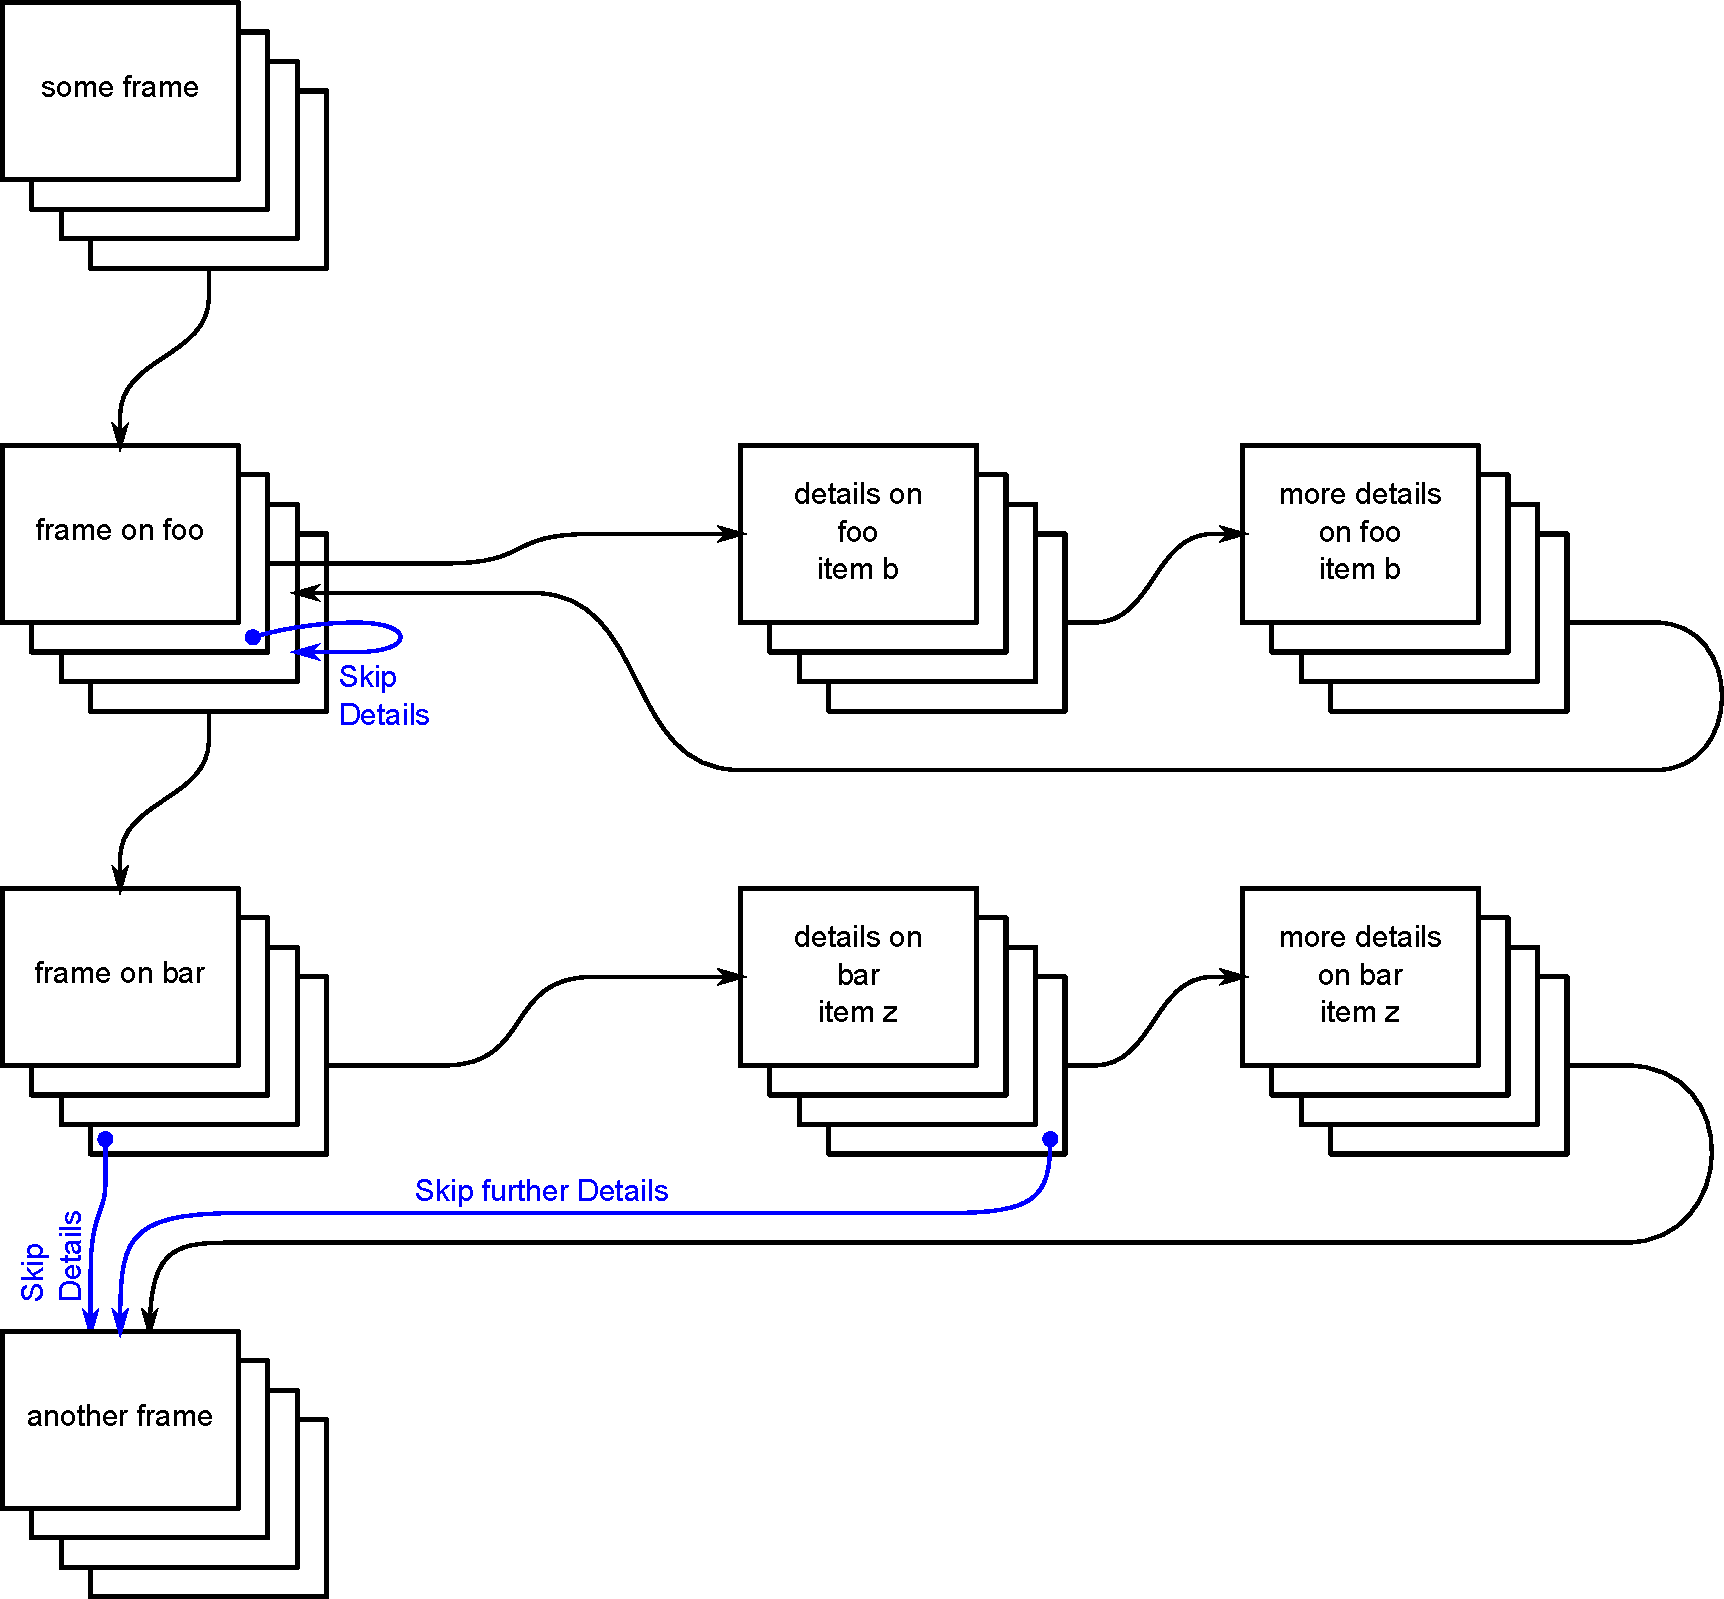
\includegraphics[width=\textwidth]{beamersubframe-embed.pdf}
% \caption{Frame Order with Details embedded}\label{fig:embed}
% \end{figure}
% 
% \begin{figure}[htb]
% 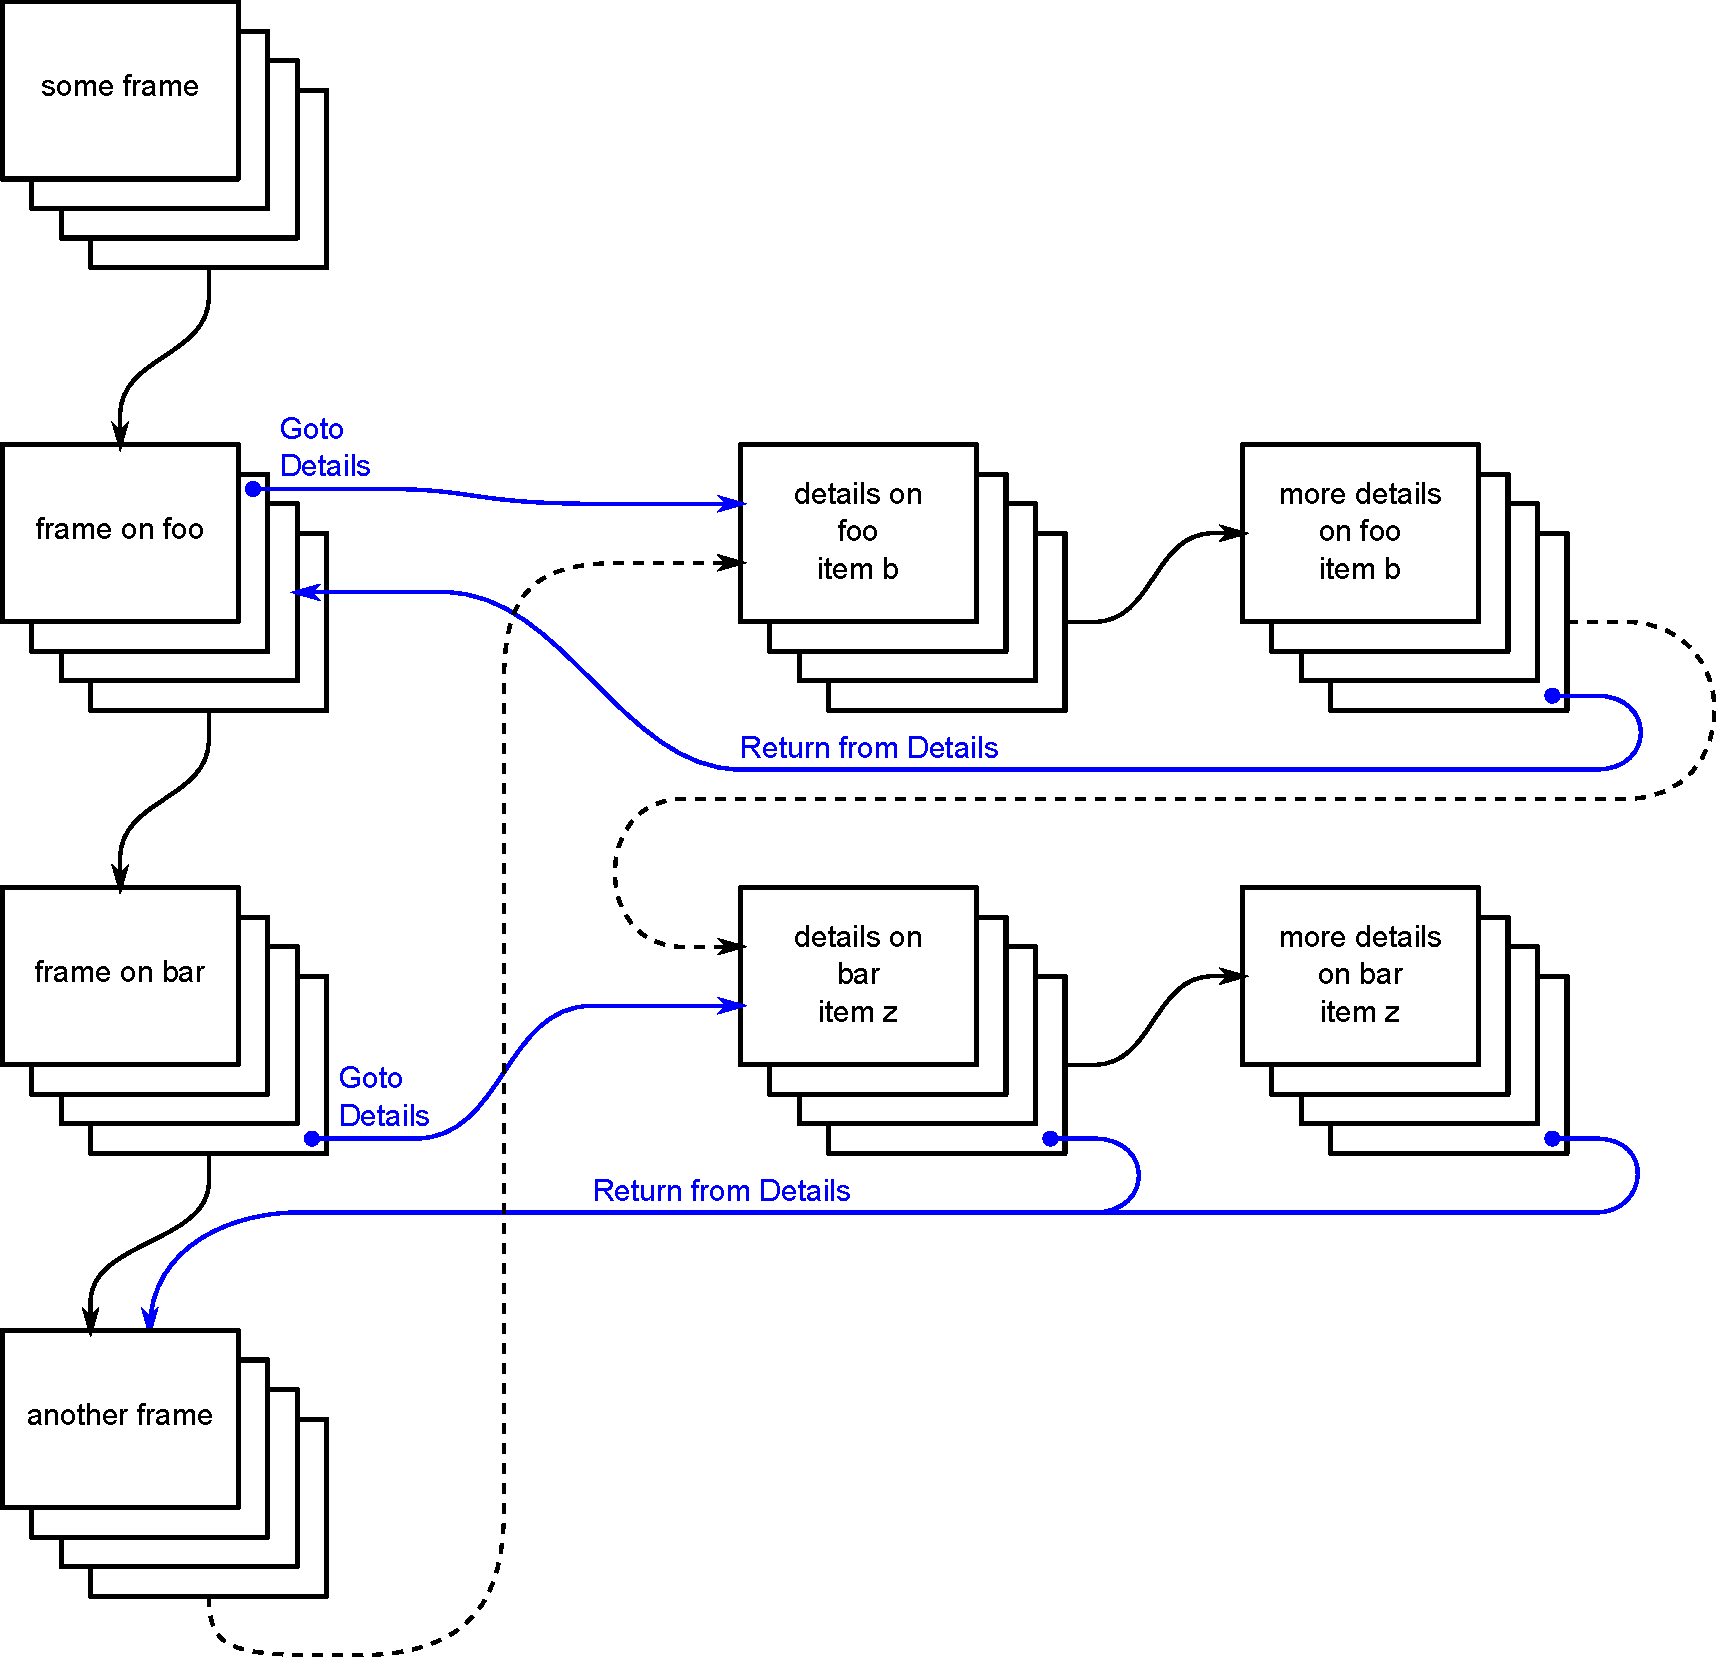
\includegraphics[width=\textwidth]{beamersubframe-append.pdf}
% \caption{Frame Order with Details appended}\label{fig:append}
% \end{figure}
% 
% Of course, the way the links are arranged in the picuters is only an example.
% There are hundreds of possibilities. And how the links are arranged the best
% way, depends on the presentation \emph{and} on the person giving the
% presentation. For this section, let's consider the links in the pictures
% the ideal way.
%
% To use the \BSF\ package, in the source the frames must be arranged as shown
% in \autoref{fig:embed}. By default, the frames in the PDF file are arranged
% the same way. By just using the option |append|, the frames in the PDF file
% will be arragned as shown in \autoref{fig:append}.
%
% ^^A---------------------------------------------
% \subsection{Basic Changes to the Source}
% To use the \BSF\ package, a few changes to the source of a presentaion must
% be applied. In the example below, the left side shows the source before the
% changes and the right side the source after them.
%
% \noindent
% \begin{minipage}{0.49\textwidth}
% \footnotesize
% \begin{verbatim}
% \begin{frame}{Frame on Foo}
% material on foo
% \end{frame}
% 
% \begin{frame}
%     {Details on Foo Item b}
% details for item b
% \end{frame}
% 
% \begin{frame}{Another Frame}
% other material
% \end{frame}
% 
% \end{document}
% \end{verbatim}
% \end{minipage}
% \hfill
% \begin{minipage}{0.49\textwidth}
% \footnotesize
% \begin{verbatim}
% \begin{frame}{Frame on Foo}
% material on foo
% \end{frame}
% 
% \begin{subframe}
%     {Details on Foo Item b}
% details for item b
% \end{subframe}
% 
% \begin{frame}{Another Frame}
% other material
% \end{frame}
% \appendsubframes
% \end{document}
% \end{verbatim}
% \end{minipage}
% 
% Here, the |frame| environment for the frame with details was changed to the
% |subframe| environment, and the command |\appendsubframes| was inserted
% before |\end{document}|. This is the minimum of changes necessary.
% 
% It is not necessary, to change the arguments of subframes. Also, there is no
% need to change the contents of subframes. Even the |fragile| option (for
% verbatim material) will work, because the |subframe| environment automatically
% adds the option |environment=subframe|.
%
% ^^A---------------------------------------------
% \subsection{Conditional Links}
% \label{sec:clinks}
% How links are used and arranged, it totally up to the user, because this is
% highly individual. But nevertheless, links in embed mode should be different
% from links in append mode. For example, a link on a frame before a subframe
% (or a group of subframes) with details should skip them in embed mode, while
% in append mode the same link should lead to the subframe (or the first
% subframe of the group).
% 
% Let's stay with the examples shown in \autoref{fig:embed} and
% \autoref{fig:append}.
% 
% The link ``Skip Details'' on slide 2 of ``frame on foo'' in embed mode is
% replaced by a link ``Goto Details'' in append mode. In the first case the
% destination is slide 3 of ``frame on foo'' and in the second case it is
% slide 1 of ``details on foo item b''.
% 
% Let's say, ``frame on foo'' has a label ``lfoo'', given as option |label=lfoo|
% to the |frame| environment (this is also necessary, if the \BSF\ package is
% not used). For append mode a label must be added to the subframe ``details
% on foo item b''. Let's call it ``ldfoob''.
% 
% For embed mode the link can be realised with
% \begin{verbatim}
% \uncover<2>{\hyperlink{lfoo<3>}{\beamerskipbutton{Skip Details}}}
% \end{verbatim}
% and for append mode with
% \begin{verbatim}
% \uncover<2>{\hyperlink{ldfoob}{\beamergotobutton{Goto Details}}}
% \end{verbatim}
% 
% In order to make the link work as expected in both modes, without the need to
% change the source, |\ifappend| can be used like this:
% \begin{verbatim}
% \ifappend{\uncover<2>{\hyperlink{ldfoob}%
%                          {\beamergotobutton{Goto Details}}}}%
%          {\uncover<2>{\hyperlink{lfoo<3>}%
%                          {\beamerskipbutton{Skip Details}}}}
% \end{verbatim}
% 
% The link to return from the frames with details can then be done this way:
% \begin{verbatim}
% \ifappend{\uncover<4>{\hyperlink{lfoo<3>}%
%                          {\beamerreturnbutton{Return from Details}}}}{}
% \end{verbatim}
% This has the disatvantage, that in embed mode there is no link, and therefore
% the layout will differ between embed mode and append mode. But this can be
% fixed by adding an invisible button like this:
% \begin{verbatim}
% \ifappend{\uncover<4>{\hyperlink{lfoo<3>}
%                          {\beamerreturnbutton{Return from Details}}}}%
%          {\visible<0>{\beamerreturnbutton{Return from Details}}}
% \end{verbatim}
% 
% Typing all this every time can be a bit exhausting. So let's define some macros.
% 
% For skipping or going to the details, a macro called |\linkdetail| can be
% defined as
% \begin{verbatim}
% \newcommand<>{\linkdetail}[4]{%
%     \ifappend{\uncover#5{\hyperlink{#3}{\beamergotobutton{#4}}}}%
%              {\uncover#5{\hyperlink{#1}{\beamerskipbutton{#2}}}}
% }
% \end{verbatim}
% 
% The command is overlay-aware and it has four arguments:
% \begin{description}
% \item[\texttt{\#1}] is the label for the destination to go to in order to skip
%       the details.
% \item[\texttt{\#2}] is the text for the link to skip the details.
% \item[\texttt{\#3}] is the label for the destination to go to in order to jump
%       to the details.
% \item[\texttt{\#4}] is the text for the link to go to the details.
% \end{description}
% Now the link on the frame before the subframe can be written as
% \begin{verbatim}
% \linkdetails<2>{lfoo<3>}{Skip Details}{ldfoob}{Goto Details}
% \end{verbatim}
% 
% For returning from the details, a macro called |\returndetail| can be
% defined as
% \begin{verbatim}
% \newcommand<>{\returndetail}[2]{%
% \ifappend{\uncover#3{\hyperlink{#1}{\beamerreturnbutton{#2}}}}%
%          {\visible<0>{\beamerreturnbutton{#2}}}
% }
% \end{verbatim}
% 
% The command is also overlay-aware and it has two arguments:
% \begin{description}
% \item[\texttt{\#1}] is the label for the destination to go to in order to return
%       from details.
% \item[\texttt{\#2}] is the text for the link to return from details.
% \end{description}
% And the link on the subframe can be written as
% \begin{verbatim}
% \returndetails<4>{lfoo<3>}{Return from Details}
% \end{verbatim}
% 
% Of course, these are only examples. How links are done, is up to the user.
% And therefore, it is also up to the user, how commands like |\linkdetail| and
% |\returndetail| are defined.
%
% Another example: I like my links to be active only on the slide, they are
% needed. On all other slides, they should be covered and inactive. So I definded
% the macros a bit different:
% \begin{verbatim}
% \newcommand<>{\linkdetail}[4]{%
%     \ifappend{\uncover#5{\alt#5{\hyperlink{#3}{\beamergotobutton{#4}}}%
%                                {\beamergotobutton{#4}}}}%
%              {\uncover#5{\alt#5{\hyperlink{#1}{\beamerskipbutton{#2}}}%
%                                {\beamerskipbutton{#2}}}}
% }
% \newcommand<>{\returndetail}[2]{%
%     \ifappend{\uncover#3{\alt#3{\hyperlink{#1}{\beamerreturnbutton{#2}}}%
%                                {\beamerreturnbutton{#2}}}}{}
% }
% \end{verbatim}
%
% ^^A---------------------------------------------
% \subsection{An Example}
% \subsubsection{Without \BSF}
% As an example, let's realise frames in the order shown in \autoref{fig:embed}
% and \autoref{fig:append}. To show the difference of the source with and
% without using the \BSF\ package, first the order shown in \autoref{fig:embed}
% is realised without \BSF.
% 
% \begin{verbatim}
% \documentclass{beamer}
% \usepackage{lmodern}
% \usepackage[T1]{fontenc}
% 
% \begin{document}
% \begin{frame}{some frame}
% \begin{itemize}[<+->]
% \item there is foo
% \item foo is good
% \item and there is bar
% \item bar is good too
% \end{itemize}
% \end{frame}
% 
% \begin{frame}<1-2>[label=lfoo]{frame on foo}
% \begin{itemize}[<+->]
% \item item a
% \item item b \uncover<2>{\hyperlink{lfoo<3>}%
%                             {\beamerskipbutton{Skip Details}}}
% \item item c
% \item item d
% \end{itemize}
% \end{frame}
% 
% \begin{frame}{details on foo item b}
% \begin{itemize}[<+->]
% \item item b.1
% \item item b.2
% \item item b.3
% \item item b.4
% \end{itemize}
% \end{frame}
% 
% \begin{frame}
% \frametitle{more details on foo item b}
% \begin{itemize}[<+->]
% \item item b.5
% \item item b.6
% \item item b.7
% \item item b.8
% \end{itemize}
% \end{frame}
% 
% \againframe<3->{lfoo}
% 
% \begin{frame}{frame on bar}
% \begin{itemize}[<+->]
% \item item w
% \item item x
% \item item y
% \item item z \uncover<4>{\hyperlink{lother}%
%                             {\beamerskipbutton{Skip Details}}}
% \end{itemize}
% \end{frame}
% 
% \begin{frame}
% \frametitle{details on bar item z}
% \begin{itemize}[<+->]
% \item item z.1
% \item item z.2
% \item item z.3
% \item item z.4
% \end{itemize}
% 
% \vspace{2ex}
% \uncover<4>{\hyperlink{lother}{\beamerskipbutton{Skip further Details}}}
% \end{frame}
% 
% \begin{frame}{more details on bar item z}
% \begin{itemize}[<+->]
% \item item z.5
% \item item z.6
% \item item z.7
% \item item z.8
% \end{itemize}
% \end{frame}
% 
% \begin{frame}[label=lother]{another frame}
% \begin{itemize}[<+->]
% \item conclusion 1
% \item conclusion 2
% \item conclusion 3
% \item conclusion 4
% \end{itemize}
% \end{frame}
% \end{document}
% \end{verbatim}
% 
% ^^A-------------------------
% \subsubsection{With \BSF}
% And now the same order of frames, but this time using the \BSF\ package and
% with some comments. 
% \begin{verbatim}
% \documentclass{beamer}
% \usepackage{lmodern}
% \usepackage[T1]{fontenc}
% \end{verbatim}
% Here, the option |embed| has to be changed to |append|, to get the order as
% shown in \autoref{fig:append}.
% \begin{verbatim}
% \usepackage[embed]{beamersubframe}
% \end{verbatim}
% The two commands, as explained in \autoref{sec:clinks}.
% \begin{verbatim}
% \newcommand<>{\linkdetail}[4]{%
%     \ifappend{\uncover#5{\hyperlink{#3}{\beamergotobutton{#4}}}}%
%              {\uncover#5{\hyperlink{#1}{\beamerskipbutton{#2}}}}
% }
% \newcommand<>{\returndetail}[2]{%
% \ifappend{\uncover#3{\hyperlink{#1}{\beamerreturnbutton{#2}}}}%
%          {\visible<0>{\beamerreturnbutton{#2}}}
% }
% \end{verbatim}
% The next command realises a link with the same destination (argument |#1|) for
% both modes, but different texts (|#2| for embed mode and |#3| for append mode.
% \begin{verbatim}
% \newcommand<>{\linkdifftext}[3]{%
%     \ifappend{\uncover#4{\hyperlink{#1}{\beamergotobutton{#3}}}}%
%              {\uncover#4{\hyperlink{#1}{\beamerskipbutton{#2}}}}
% }
% \end{verbatim}
% The template defined below is an example for the use of |\ifsubframe|. It puts
% the text ``detail'' in the lower left corner of subframes and ``main part'' in
% the lower left corner of normal frames. Careful: it replaces a sidebar, so
% this will not work with themes like Berkeley.
% \begin{verbatim}
% \defbeamertemplate*{sidebar left}{bsf test}[1][50]
% {
%   \vfill%
%   \rlap{\hskip0.1cm\hbox{\color{fg!#1!bg}\tiny{\ifsubframe{detail}{main part}}}}%
%   \vskip2pt%
% }
% 
% \begin{document}
% \begin{frame}{some frame}
% \begin{itemize}[<+->]
% \item there is foo
% \item foo is good
% \item and there is bar
% \item bar is good too
% \end{itemize}
% \end{frame}
% 
% \begin{frame}<1-2>[label=lfoo]{frame on foo}
% \begin{itemize}[<+->]
% \item item a
% \end{verbatim}
% Here, the link was changed.
% \begin{verbatim}
% \item item b \linkdetail<2>{lfoo<3>}{Skip Details}{ldfoob}{Goto Details}
% \item item c
% \item item d
% \end{itemize}
% \end{frame}
% \end{verbatim}
% For the next two frames the environment was changed to |subframe|. And for the
% first, the label |ldfoob| was added.
% \begin{verbatim}
% \begin{subframe}[label=ldfoob]{details on foo item b}
% \begin{itemize}[<+->]
% \item item b.1
% \item item b.2
% \item item b.3
% \item item b.4
% \end{itemize}
% \end{subframe}
% 
% \begin{subframe}
% \frametitle{more details on foo item b}
% \begin{itemize}[<+->]
% \item item b.5
% \item item b.6
% \item item b.7
% \item item b.8
% \end{itemize}
% 
% \vspace{2ex}
% \end{verbatim}
% The link to return from details was added. Because there was no link in the
% version without \BSF\ the layout of the frame is now changed compared to that
% version. But it doesn't change from one mode to the other, because of the way
% |\returndetails| was definded.
% \begin{verbatim}
% \returndetail<4>{lfoo<3>}{Return from Details}
% \end{subframe}
% 
% \againframe<3->{lfoo}
% 
% \begin{frame}{frame on bar}
% \begin{itemize}[<+->]
% \item item w
% \item item x
% \item item y
% \end{verbatim}
% Again, the link was changed here.
% \begin{verbatim}
% \item item z \linkdetail<4>{lother}{Skip Details}{ldbarz}{Goto Details}
% \end{itemize}
% \end{frame}
% \end{verbatim}
% For the next two frames the environment was changed to |subframe| also. And
% for the first, the label |ldbarz| was added.
% \begin{verbatim}
% \begin{subframe}[label=ldbarz]
% \frametitle{details on bar item z}
% \begin{itemize}[<+->]
% \item item z.1
% \item item z.2
% \item item z.3
% \item item z.4
% \end{itemize}
% 
% \vspace{2ex}
% \end{verbatim}
% This link was changed, so the text differs between modes. But it would have
% been possible here, to leave the link unchanged.
% \begin{verbatim}
% \linkdifftext<4>{lother}{Skip further Details}{Return from Details}
% \end{subframe}
% 
% \begin{subframe}{more details on bar item z}
% \begin{itemize}[<+->]
% \item item z.5
% \item item z.6
% \item item z.7
% \item item z.8
% \end{itemize}
% 
% \vspace{2ex}
% \end{verbatim}
% Again, the link was added here, resulting also in a change off layout compared
% to the first version.
% \begin{verbatim}
% \returndetail<4>{lother}{Return from Details}
% \end{subframe}
% 
% \begin{frame}[label=lother]{another frame}
% \begin{itemize}[<+->]
% \item conclusion 1
% \item conclusion 2
% \item conclusion 3
% \item conclusion 4
% \end{itemize}
% \end{frame}
% \end{verbatim}
% And finally, the |\appendsubframes| command was inserted here.
% \begin{verbatim}
% \appendsubframes
% \end{document}
% \end{verbatim}
% 
% The source of the second version is available as example file, which can be
% generated from |beamersubframe.dtx|.
%
% ^^A--------------------------------------------------------------------------
% \section{Restrictions}
% \label{sec:restrictions}
% Since this is an early version of the \BSF\ package, there are some
% restrictions.
%
% \begin{itemize}
% \item The package was only tested with Beamer mode |beamer|. Using other
%       modes may lead to strange errors.
% \item Supporting material, like notes, is not tested yet.
% \item Lectures are not tested yet.
% \item There is no support for subsubsections (not even tested). And it is not
%       planned at all.
% \item There is no |\subframe| command.
% \item There is no |\againsubframe| command.
% \end{itemize}
% 
% ^^A--------------------------------------------------------------------------
% \section{Testing}
% For testing the \BSF\ package the following themes were used:
% \begin{itemize}
% \item Dresden
% \item Darmstadt
% \item Berkeley
% \item Montpellier
% \item Malmoe
% \item AnnArbor
% \end{itemize}
% 
% The themes were used without options. They where choosen to cover all types of
% navigation possible with the themes delivered with Beamer. If I missed
% something and this doesn't work, please let me know. If there are other things
% not working (e.g.\ some inserts), please let me know too. In both cases, a
% file for testing would be nice.
%
% ^^A--------------------------------------------------------------------------
% \section{ToDo}
% Although the \BSF\ package is already useful, there are a lot of things left
% to do:
% \begin{description}
% \item[testing] Beamer has a lot of features, an many of them are still
%       not tested.
% \item[Beamer modes] I have to admit, I didn't even test them.
% \item[notes] The same here.
% \item[lectures] And again, not tested.
% \item[macros] There are commands, which would be nice to have, like
%       |\subframe|, |\againsubframe|, and |\subnote| (to get notes between
%       frames moved too)
% \item[levels] With multiple levels of subframes, it would be possible, to have
%       details on details (on details on \dots). And then, one could embed the
%       first $n$ levels of details, and append the others.
% \end{description}
% 
% The list is not complete. If someone has an item to add, please let me know.
%
% ^^A--------------------------------------------------------------------------
% \StopEventually{\newpage\PrintIndex}
% ^^A \PrintChanges}
%
% ^^A--------------------------------------------------------------------------
% \newpage
% \section{The Code}
% \subsection{The Usual}
% First the usual things.
%    \begin{macrocode}
\NeedsTeXFormat{LaTeX2e}
\ProvidesPackage{beamersubframe}[\filedate\space
    v\fileversion\space reordering beamer frames]
%    \end{macrocode}
%
% ^^A---------------------------------------------
% \subsection{Check the Class}
% Since the \BSF\ package only works with the Beamer class and article mode is
% not supported yet, check for the Beamer class. If it is not loaded, throw an
% error message and stop loading the package.
%    \begin{macrocode}
\@ifclassloaded{beamer}{}{%
  \PackageError{beamersubframe}{%
    The package works only with the beamer class,\MessageBreak
    therefore it is not loaded.
  }{%
    The package is not loaded, because it needs the\MessageBreak
    beamer class. Continuing may lead to additional\MessageBreak
    errors because of undefined commands.
  }
  \endinput
}
%    \end{macrocode}
%
% ^^A---------------------------------------------
% \subsection{``Variables''}
% \begin{macro}{\if@bsf@append}
% First there is the main flag to distinguish between append mode and embed mode.
%    \begin{macrocode}
\newif\if@bsf@append
%    \end{macrocode}
% \end{macro}
%
% \begin{macro}{\if@bsf@miniframes}
% This flag is true by default. It is set to false by the option |nominiframes|.
%    \begin{macrocode}
\newif\if@bsf@miniframes
\@bsf@miniframestrue
%    \end{macrocode}
% \end{macro}
%
% \begin{macro}{\if@bsf@subframe}
% This flag is set to true for subframes in both modes. For normal frames it is
% false.
%    \begin{macrocode}
\newif\if@bsf@subframe
\@bsf@subframefalse
%    \end{macrocode}
% \end{macro}
%
% \begin{macro}{\if@bsf@nosfnum}
% This flag is used for checking the |.sfp| file.
%    \begin{macrocode}
\newif\if@bsf@nosfnum
%    \end{macrocode}
% \end{macro}
%
% \begin{macro}{\if@bsf@firstline}
% This flag is needed to write |\begin{frame}| in front of the arguments of a
% |subframe| environment to the |.sfr| file in append mode.
%    \begin{macrocode}
\newif\if@bsf@firstline
%    \end{macrocode}
% \end{macro}
%
% \begin{macro}{\if@bsf@firstpart}
% This flag is needed by |\bsfrestorepart| to initialize some macros used as
% variables instead of writing the |\bsf@partpages| entry to the |.nav| file.
%    \begin{macrocode}
\newif\if@bsf@firstpart
%    \end{macrocode}
% \end{macro}
%
% \begin{macro}{\if@bsf@firstsection}
% This flag is needed by |\bsfrestoresection| to initialize some macros used as
% variables instead of writing the |\bsf@sectionpages| entry to the |.nav| file.
%    \begin{macrocode}
\newif\if@bsf@firstsection
%    \end{macrocode}
% \end{macro}
%
% \begin{macro}{\if@bsf@firstsubsection}
% This flag is needed by |\bsfrestoresubsection| to initialize some macros used
% as variables instead of writing the |\bsf@subsectionpages| entry to the |.nav|
% file.
%    \begin{macrocode}
\newif\if@bsf@firstsubsection
%    \end{macrocode}
% \end{macro}
%
% \begin{macro}{\if@bsf@nosubsection}
% This flag is used by |\bsfrestoresection| and |\bsfrestoresubsection| to
% determine, if a section contains any subsections.
%    \begin{macrocode}
\newif\if@bsf@nosubsection
%    \end{macrocode}
% \end{macro}
%
% \begin{macro}{\if@bsf@prevnosubsection}
% This flag contains the final state of |\if@bsf@nosubsection| for the previous
% section.
%    \begin{macrocode}
\newif\if@bsf@prevnosubsection
%    \end{macrocode}
% \end{macro}
%
% \begin{macro}{\bsf@frame@param}
% This token register is used to store the first three arguments of the
% |subframe| environment in embed mode, after adding the option
% |environmet=subframe|. The contents is passed to the |frame| environmet as
% its first three arguments.
%    \begin{macrocode}
\newtoks\bsf@frame@param
%    \end{macrocode}
% \end{macro}
%
% \begin{macro}{\bsf@sfrout}
% The stream used to write the |.sfr| file. It holds the contents of all
% subframes. The file is only written and used in append mode.
%    \begin{macrocode}
\newwrite\bsf@sfrout
%    \end{macrocode}
% \end{macro}
%
% ^^A---------------------------------------------
% \subsection{Options and Packages}
% \begin{option}{embed}
% The options are rather simple. The option |embed| just sets |\if@bsf@append|
% to false.
%    \begin{macrocode}
\DeclareOption{embed}{\@bsf@appendfalse}
%    \end{macrocode}
% \end{option}
% \begin{option}{append}
% And |append| sets |\if@bsf@append| to true.
%    \begin{macrocode}
\DeclareOption{append}{\@bsf@appendtrue}
%    \end{macrocode}
% \end{option}
% \begin{option}{nominiframes}
% The option |nominiframes| sets |\if@bsf@miniframes| to false.
%    \begin{macrocode}
\DeclareOption{nominiframes}{\@bsf@miniframesfalse}
%    \end{macrocode}
% \end{option}
% The default is set and the options are processed.
%    \begin{macrocode}
\ExecuteOptions{embed}
\ProcessOptions*\relax
%    \end{macrocode}
% And the verbatim package is loaded.
%    \begin{macrocode}
\RequirePackage{verbatim}
%    \end{macrocode}

% ^^A---------------------------------------------
% \subsection{Navigation}
% \subsubsection{Sidebar and Headline}
% To get the highlighting of sections and subsections on appened subframes as if
% the frames were embedded, some counters must be restored to the values, they
% had at the point, the subframe appeared in the source. Additionally, for the
% headline some inserts must be restored.
% 
% To achieve this, the |subframe| environment writes a macro with all necessary
% arguments to the |.sfr| file. This is done for each subframe, before its
% contents, embedded in a |frame| environmet, is written to the file (see
% \autoref{sec:code-subframe}).
% 
% \begin{macro}{\bsfrestore}
% The macro is called |\bsfrestore|. It is executed, when the |.sfr| file is
% loaded. It restores the counters for part (|#1|), section (|#2|), and
% aubsection (|#3|). It also restores the counter subsectionslide (|#4|), which
% is needed for miniframes.
% 
% Then |\insertsectionhead| and |\insertsubsectionhead| are restored to their
% meanings at the point, the subframe appeard in the source. These meanings were
% stored to the two macros |\bsf@sectionhead|\meta{part}|.|\meta{section} and
% |\bsf@subsectionhead|\meta{part}|.|\meta{section}|.|\meta{subsection} by the
% |subframe| environment (see \autoref{sec:code-subframe}).
% 
% After that, the inserts for the part, section, and subsection numbers are
% restored.
% 
% The macro is also used by the |lastframe| environment (see
% \autoref{sec:code-lastframe}).
%    \begin{macrocode}
\newcommand{\bsfrestore}[4]{%
  \setcounter{part}{#1}%
  \setcounter{section}{#2}%
  \setcounter{subsection}{#3}%
  \setcounter{subsectionslide}{#4}%
  \expandafter\let\expandafter\insertsectionhead
    \csname bsf@sectionhead\the\c@part.\the\c@section\endcsname
  \expandafter\let\expandafter\insertsubsectionhead
    \csname bsf@subsectionhead\the\c@part.\the\c@section.\the\c@subsection\endcsname
  \def\insertpartheadnumber{#1}%
  \def\insertsectionheadnumber{#2}%
  \def\insertsubsectionheadnumber{#3}%
}
%    \end{macrocode}
% \end{macro}
% 
% ^^A-------------------------
% \subsubsection{Miniframes}
% \label{sec:code-miniframes}
% To typset miniframes, Beamer writes a |\slideentry| with the necessary
% arguments to the |.nav| file. Because miniframes should appear, as if the
% subframes are embedded, the |subframe| environment has to write such an entry
% at the point, the subframe appears in the source. But instead of a
% |\slideentry|, \BSF\ writes a |\subslideentry| (see \autoref{sec:man-subse}).
% 
% Argument |#4| of |\slideentry| contains the start page and the end page of the
% frame. Unfortunately, for subframes these numbers are unknown, until the
% |.sfr| file was loaded by |\appendsubframes|.
% 
% To get around this, for each subframe two macros are used. Their names \linebreak
% are
% |\bsf@substartpage|\meta{part}|.|\meta{section}|.|\meta{subsection}|.|\meta{subsectionslide}
% and \linebreak
% |\bsf@subendpage|\meta{part}|.|\meta{section}|.|\meta{subsection}|.|\meta{subsectionslide}.
% Here \meta{part}, \meta{section} and so on are the numbers.
% 
% Now at the point where the subframe appears in the souce, the |\subslideentry|
% is written. Instead of the unknown frame numbers, it contains the sequence
% |{\bsf@usenum{bsf@substartpage...}/\bsf@usenum{bsf@subendpage...}}| as argument
% |#4|. After a subframe was typeset by loading the |.sfr| file, the necessary
% information is written to the |.sfp| file. In the next \TeX\ run, when loading
% the |.sfp| file at the beginning of the document (see \autoref{sec:code-beginend}),
% these macros are all defined.
% 
% \begin{macro}{\bsf@subnum}
% The first macro involved is just a shortcut to get the numbers.
%    \begin{macrocode}
\def\bsf@subnum{%
  \the\c@part.\the\c@section.\the\c@subsection.\the\c@subsectionslide
}
%    \end{macrocode}
% \end{macro}
% 
% Beamer uses the macro |\beamer@writeslidentry| to write the |\slideentry| and
% the |\beamer@framepages| entry (used for the navigation bar) to the |.nav|
% file. For subframes this is split into two macros.
% 
% \begin{macro}{\beamer@writeslidentry@miniframes}
% The |\subslideentry| is written by |\beamer@writeslidentry@miniframes|. The
% macro is called directly by the |subframe| environment (see
% \autoref{sec:code-subframe}).
%    \begin{macrocode}
\def\beamer@writeslidentry@miniframes{%
  \addtocontents{nav}%
    {\protect\headcommand{%
      \protect\subslideentry{\the\c@section}{\the\c@subsection}%
        {\the\c@subsectionslide}%
        {\protect\bsf@usenum{bsf@substartpage\bsf@subnum}/%
         \protect\bsf@usenum{bsf@subendpage\bsf@subnum}}%
        {\lastsubsection}{\the\c@part}}}%
}
%    \end{macrocode}
% \end{macro}
% 
% \begin{macro}{\beamer@writeslidentry@navbar}
% The |\beamer@framepages| entry is written by |\beamer@writeslidentry@navbar|.
% And it also writes the |\bsfsubframepages| entry to the |.sfp| file.
% 
% This macro is used to replace |\beamer@writeslidentry|, before the |.sfr| file
% is loaded. This is done in |\appendsubframes| (see \autoref{sec:code-appendsub}).
%    \begin{macrocode}
\def\beamer@writeslidentry@navbar{%
  \expandafter\beamer@ifempty\expandafter{\beamer@framestartpage}{}% does not happen normally
  {%else
    \addtocontents{nav}%
      {\protect\headcommand{% 
        \protect\beamer@framepages{\beamer@framestartpage}{\beamer@frameendpage}}}%
    \addtocontents{sfp}{%
      \protect\bsfsubframepages{\the\c@part}{\the\c@section}{\the\c@subsection}%
        {\the\c@subsectionslide}{\beamer@framestartpage}{\beamer@frameendpage}}%
    \clearpage\beamer@notesactions%
  }%
}
%    \end{macrocode}
% \end{macro}
% 
% \begin{macro}{\subslideentry}
% The |\subslideentry| is initialized in a way that it does the same as the
% |\slideentry|. Because |\slideentry| is refedined by some themes, |\let| can
% not be used here.
%    \begin{macrocode}
\def\subslideentry{\slideentry}
%    \end{macrocode}
% \end{macro}
% 
% \begin{macro}{\bsfsubframepages}
% The |.sfp| file contains one |\bsfsubframepages| entry for each subframe. The
% arguments are the part number (|#1|), the section number (|#2|), the subsection
% number (|#3|), the subsectionslide number (|#4|), and the first (|#5|) and the
% last page of the subframe (|#6|).
% 
% When the |.sfp| file is loaded, each |\bsfsubframepages| defines two macros
% |\bsf@substartpage...| and |\bsf@subendpage...| used by the |\subslideentry|.
%    \begin{macrocode}
\def\bsfsubframepages#1#2#3#4#5#6{%
  \expandafter\def\csname bsf@substartpage#1.#2.#3.#4\endcsname{#5}%
  \expandafter\def\csname bsf@subendpage#1.#2.#3.#4\endcsname{#6}%
}
%    \end{macrocode}
% \end{macro}
%
% \begin{macro}{\bsf@usenum}
% The macro |\bsf@usenum|, used in the |\subslideentry|, sets a default in case
% the |\bsf@substartpage...| and |\bsf@subendpage...| macros are not defined due
% to a missing, corrupted or incomplete |.sfp| file. Without this, there could
% be errors which would persist on every subsequent run of \TeX.
%    \begin{macrocode}
\def\bsf@usenum#1{%
  \@ifundefined{#1}{1}{\csname #1\endcsname}%
}
%    \end{macrocode}
% \end{macro}
%
% \begin{macro}{\bsf@checksfp}
% In order to warn the user about a missing, corrupted or incomplete |.sfp| file,
% the file is checked. This is done indirectly by checking, if all
% |\bsf@substartpage...| and |\bsf@subendpage...| macros in the current |.nav|
% file are defined. 
% 
% For this all commands in the |.nav| file are executed using Beamers |\dohead|
% command. Because some of the commands would typeset something, they are
% disabled and everything is done in a group to keep the changes local.
% 
% The macro |\bsf@usenum| is also redefined to set the flag |\if@bsf@nosfnum| to
% true in case one of the checked macros is undefined.
%    \begin{macrocode}
\def\bsf@checksfp{%
  \begingroup
    \@bsf@nosfnumfalse
    \def\bsf@usenum##1{%
      \@ifundefined{##1}{\@bsf@nosfnumtrue}{}}
    \def\slideentry##1##2##3##4##5##6{}%
    \def\partentry##1##2{}%
    \def\sectionentry##1##2##3##4##5{}%
    \def\beamer@subsectionentry##1##2##3##4##5{}%
    \def\subslideentry##1##2##3##4##5##6{%
      \bsf@checksfnum(##4)}%
    \dohead
    \if@bsf@nosfnum
      \PackageWarningNoLine{Beamer SubFrame}{%
        Missing, incomplete or corrupted file\MessageBreak
        \jobname.sfp! Links for miniframes of\MessageBreak
        subframes may be wrong. Please run TeX\MessageBreak
        again}
    \fi
  \endgroup
}
%    \end{macrocode}
% \end{macro}
%
% \begin{macro}{\bsf@checksfnum}
% The macro |\bsf@checksfnum| is just used by |\bsf@checksfp| to get rid of the
% slash in argument |#4| of the |\subslideentry|.
%    \begin{macrocode}
\def\bsf@checksfnum(#1/#2){#1#2}
%    \end{macrocode}
% \end{macro}
% 
% ^^A-------------------------
% \subsubsection{Navigation Bar}
% Getting the navigation bar right takes some effort. First lets take a look,
% what Beamer does to get the necessary information for the navigation bar.
% 
% \paragraph{How Beamer does it}~\\
% Beamer writes several different entries to the |.nav| file.
% \begin{description}
% \item[\texttt{\bslash beamer@framepages}] with the first and the last page of
%       the frame as arguments. It is written for every frame at its end.
% \item[\texttt{\bslash beamer@subsectionpages}] with the first and the last
%       page of the subsection as arguments. It is written by the |\subsection|
%       command for the previous subsection, as well as by |\section| and
%       |\part| and the end of the document for the last subsection.
% \item[\texttt{\bslash beamer@sectionpages}] with the first and the last page
%       of the section as arguments. It is written by the |\section| command for
%       the previous section, as well as by |\part| and the end of the document
%       for the last section.
% \item[\texttt{\bslash beamer@partpages}] with the first and the last page of
%       the part as arguments. It is written by the |\part| command for the
%       previous part and the end of the document for the last part.
% \item[\texttt{\bslash beamer@documentpages}] with the last page of the
%       documnet as argument. It is written at the end of the document.
% \end{description}
% 
% The macros in the |.nav| file are executed once for every page (i.e.\ slide).
% By this the entry |\beamer@framepages| sets the macro |\beamer@startpageofframe|
% to its first argument and |\beamer@endpageofframe| to its second argument, but
% only if the current page is $\ge$ than the first argument and $\le$ than the
% second one. Similar macros are set the same way by the other entries. 
% 
% The frame icon is then typeset in a way, that
% \begin{itemize}
% \item the left arrow points to page |\beamer@startpageofframe| $-1$,
% \item the left part of the frame symbol points to page |\beamer@startpageofframe|,
% \item the right part of the frame symbol points to page |\beamer@endpageofframe|,
% \item and the right arrow points to page |\beamer@endpageofframe| $+1$.
% \end{itemize}
% The arrows are limited 1 or |\beamer@endpageofdocument| respectively. The icons
% for subsections and sections are typeset in a similar way.
% 
% The right part of the presentation symbol or (if there is an appendix) of the
% appendix symbol will point to page |\beamer@endpageofdocument|.

% \paragraph{How \BSF\ does it}~\\
% The frame icon should point to the previous or next frame or subframe in the
% PDF file. This is simply achieved by writing the |\beamer@framepages| entry
% with |\beamer@writeslidentry@navbar| (see \autoref{sec:code-miniframes}) for
% every subframe.
%
% The section icon should point to the first and last page of the section the
% subframe belongs to in the main part. For this, the first page of the first
% and the last page of the last subframe of a section is needed also. The
% information is stored in two steps.
% \begin{enumerate}
% \item A macro |\bsfrestoresection| is written to the |.sfr| file for each
%       section. Its arguments are the number of the previous section and the
%       first page of the section just started.
% \item When loading the |.sfr| file, the first |\bsfrestoresection| entry
%       initializes some makros (used as variables). All subsequent entries
%       write a |\bsf@sectionpages| entry to the |.nav| file, which has the
%       necessary pages as arguments.
% \end{enumerate}
% For parts and subsections corresponding entries are written to the files. And
% for the last part, section, and subsection |\bsf@...pages| entries are written
% after appending the subframes.
% 
% The |\beamer@...pages| entries written by Beamer at the end of the document
% would mix up the links of the navigation bar. It is not possible to prevent
% writing these entries. Instead they are disabled after appending the subframes.
% Since they would stay disabled for all pages after the first, they are
% reenabled at the beginning of the |.nav| file. Also, these entries have to be
% written before appending the subframes, in order to make the navigation bar
% work correctly for the last section and subsection in the main part.
% 
% Since this is also done for the |\beamer@documentpages| entry, the right
% arrows of the section and subsection icons are limited to the last page of the
% main part, i.e.\ the page before the first subframe. The same applies to the
% right part of the presentation or appendix symbol.
% 
% Unfortunately, this would apply to the right arrows of the slide icon and the
% frame icon too. Therefore the package writes a |\bsf@documentpages| entry to
% the |.nav| file after appending the subframes. Additionally, two macros of
% Beamer are redefined to use this information, instead of the information of
% the |\beamer@documentpages| entry.
%
% \paragraph{The Macros}~\\
% Lets start with the two redefined macros. The originals are defined in
% \textsf{beamerbasenavigation.sty}.
% 
% \begin{macro}{\hyperlinkslidenext}
% The new definition of |\hyperlinkslidenext| uses |\bsf@nextpage| instead of
% |\beamer@nextpage|.
%    \begin{macrocode}
\def\hyperlinkslidenext{%
  \bsf@nextpage\c@page%
  \hyperlink{Navigation\the\beamer@tempcount}}
%    \end{macrocode}
% \end{macro}
% 
% \begin{macro}{\hyperlinkframestartnext}
% The new definition of |\hyperlinkframestartnext| also uses |\bsf@nextpage|
% instead of |\beamer@nextpage|.
%    \begin{macrocode}
\def\hyperlinkframestartnext{%
  \bsf@nextpage\beamer@endpageofframe%
  \hyperlink{Navigation\the\beamer@tempcount}}
%    \end{macrocode}
% \end{macro}
% 
% \begin{macro}{\bsf@nextpage}
% The macro |\bsf@nextpage| works like |\beamer@nextpage| (from
% \textsf{beamerbasenavigation.sty}), but it uses |\bsf@endpageofdocument| as
% the last page for links, instead of |\beamer@endpageofdocument|.
%    \begin{macrocode}
\def\bsf@nextpage#1{%
  \beamer@tempcount=#1%
  \advance\beamer@tempcount by1\relax%
  \ifnum\beamer@tempcount>\bsf@endpageofdocument%
  \beamer@tempcount=\bsf@endpageofdocument%
  \fi}
%    \end{macrocode}
% \end{macro}
% 
% \begin{macro}{\bsf@documentpages}
% The |\bsf@endpageofdocument| is defined by the |\bsf@documentpages| entry of
% the |.nav| file.
%    \begin{macrocode}
\def\bsf@documentpages#1{\def\bsf@endpageofdocument{#1}}
%    \end{macrocode}
% \end{macro}
% 
% \begin{macro}{\bsf@endpageofdocument}
% And |\bsf@endpageofdocument| is initialized to reflect the original.
%    \begin{macrocode}
\def\bsf@endpageofdocument{\beamer@endpageofdocument}
%    \end{macrocode}
% \end{macro}
% 
% To disable and reenable the |\beamer@...pages| entries, first
% \begin{macro}{\beamer@partpages@orig}
% the macro |\beamer@partpages|,
%    \begin{macrocode}
\let\beamer@partpages@orig\beamer@partpages
%    \end{macrocode}
% \end{macro}
%
% \begin{macro}{\beamer@subsectionpages@orig}
% the macro |\beamer@subsectionpages|,
%    \begin{macrocode}
\let\beamer@subsectionpages@orig\beamer@subsectionpages
%    \end{macrocode}
% \end{macro}
%
% \begin{macro}{\beamer@sectionpages@orig}
% the macro |\beamer@sectionpages|,
%    \begin{macrocode}
\let\beamer@sectionpages@orig\beamer@sectionpages
%    \end{macrocode}
% \end{macro}
%
% \begin{macro}{\beamer@documentpages@orig}
% and the macro |\beamer@documentpages| are saved.
%    \begin{macrocode}
\let\beamer@documentpages@orig\beamer@documentpages
%    \end{macrocode}
% \end{macro}
%
% \begin{macro}{\bsf@enablenaventries}
% The command |\bsf@enablenaventries| restores the original meanings of the
% |\beamer@...pages| entries. It is written to the |.nav| file at the beginning
% of the document (see \autoref{sec:code-beginend}).
%    \begin{macrocode}
\def\bsf@enablenaventries{%
  \let\beamer@partpages\beamer@partpages@orig
  \let\beamer@subsectionpages\beamer@subsectionpages@orig
  \let\beamer@sectionpages\beamer@sectionpages@orig
  \let\beamer@documentpages\beamer@documentpages@orig
}
%    \end{macrocode}
% \end{macro}
%
% \begin{macro}{\bsf@disablenaventries}
% And |\bsf@disablenaventries| disables the entries by letting them gobble their
% arguments. It is written to the |.nav| file after appending the subframes (see
% \autoref{sec:code-appendsub}).
%    \begin{macrocode}
\def\bsf@disablenaventries{%
  \let\beamer@partpages\@gobbletwo
  \let\beamer@subsectionpages\@gobbletwo
  \let\beamer@sectionpages\@gobbletwo
  \let\beamer@documentpages\@gobble
}
%    \end{macrocode}
% \end{macro}
%
% In order to write the |\bsfrestore...| entries to the |.sfr| file, the
% sectioning commands must be extended. First the originals for
%
% \begin{macro}{\part@orig}
% the macro |\part|,
%    \begin{macrocode}
\let\part@orig\part
%    \end{macrocode}
% \end{macro}
% 
% \begin{macro}{\section@orig}
% the macro |\section|,
%    \begin{macrocode}
\let\section@orig\section
%    \end{macrocode}
% \end{macro}
% 
% \begin{macro}{\subsection@orig}
% and the macro |\subsection| are saved.
%    \begin{macrocode}
\let\subsection@orig\subsection
%    \end{macrocode}
% \end{macro}
% The sectioning macros are only redefined in append mode.
%    \begin{macrocode}
\if@bsf@append
%    \end{macrocode}
% 
% \begin{macro}{\part}
% The new version of |\part| writes the |\bsfrestorepart| entry to the |.sfr|
% file. The original version is called at the end, so its arguments are of no
% concern here. But because of that, |\c@part| still contains the number of the
% previous part. Here, |\c@page| already contains the number of the first page
% of the new part.
%    \begin{macrocode}
  \def\part{%
    \immediate\write\bsf@sfrout{\string\bsfrestorepart{\the\c@part}%
        {\the\c@page}}%
    \part@orig
  }
%    \end{macrocode}
% \end{macro}
% 
% \begin{macro}{\section}
% The new version of |\section| writes the |\bsfrestoresection| entry to the
% |.sfr| file. Besides that, it works like the new |\part| command.
%    \begin{macrocode}
  \def\section{%
    \immediate\write\bsf@sfrout{\string\bsfrestoresection{\the\c@section}%
        {\the\c@page}}%
    \section@orig
  }
%    \end{macrocode}
% \end{macro}
% 
% \begin{macro}{\subsection}
% And the new version of |\subsection| writes the |\bsfrestoresubsection| entry
% to the |.sfr| file. It also works like the new |\part| command.
%    \begin{macrocode}
  \def\subsection{%
    \immediate\write\bsf@sfrout{\string\bsfrestoresubsection{\the\c@subsection}%
        {\the\c@page}}%
    \subsection@orig
  }
\fi
%    \end{macrocode}
% \end{macro}
% 
% The |\bsfrestore...| entries are executed, when loading the |.sfr| file.
% Basically, they write the |\bsf@... pages| entries to the |.nav| file. But
% the first time, they just initialize some macros used as variables, because
% at this point only the first page of the first subframe of a part, section
% or subsection and the first page of the part, section or subsection itself
% are known.
% 
% \begin{macro}{\bsfrestorepart}
% On the first call, |\bsfrestorepart| stores the the first page of the new part
% (|#2|), the number of the previous part (|#1|), and the number of the first
% page of the first subframe belonging to the new part (|c@page|).
%    \begin{macrocode}
\def\bsfrestorepart#1#2{%
  \if@bsf@firstpart
    \@bsf@firstpartfalse
    \def\bsf@partstartpage{#2}%
    \def\bsf@prevpart{#1}%
    \edef\bsf@partfirstsubframepage{\the\c@page}%
  \else
%    \end{macrocode}
% On all subsequent calls, if there is a new part, the last page of the last
% subframe belonging to the previous part (in |\@tempcnta|) and the last page
% of the previous part (in |\@tempcntb|) are calculated. 
%    \begin{macrocode}
    \@tempcnta=\bsf@prevpart\relax
    \ifnum#1>\@tempcnta
      \@tempcnta\c@page\advance\@tempcnta -1\relax
      \@tempcntb=#2\relax\advance\@tempcntb -1\relax
%    \end{macrocode}
% Then the |\bsf@partpages| entry is written to the |.nav| file. Here
% |\addtocontents| can not be used, because it doesn't work, if |\bsfrestorepart|
% appears after the last subframe.
%    \begin{macrocode}
      \if@filesw
        \immediate\write\@auxout{\string\@writefile{nav}%
          {\noexpand\headcommand{%
            \noexpand\bsf@partpages{\bsf@partfirstsubframepage}%
              {\the\@tempcnta}{\bsf@partstartpage}{\the\@tempcntb}}}}%
      \fi
%    \end{macrocode}
% After that, the ``variables'' are reinitialized.
%    \begin{macrocode}
      \def\bsf@partstartpage{#2}%
      \def\bsf@prevpart{#1}%
      \edef\bsf@partfirstsubframepage{\the\c@page}%
    \fi
  \fi
}
%    \end{macrocode}
% Two of the ``variables'' must be initialized, in order to make the package
% work for presentations without sectioning commands.
%    \begin{macrocode}
\def\bsf@partstartpage{1}%
\def\bsf@prevpart{0}%
%    \end{macrocode}
% \end{macro}
% 
% \begin{macro}{\bsfrestoresection}
% The macros |\bsfrestoresection| and |\bsfrestoresubsection| work the same way
% as |\bsfrestorepart|. But additionally, they must keep track of sections
% without subsections. For this, the flags |\if@bsf@nosubsection| and
% |\if@bsf@prevnosubsection| and the macro |\bsf@prevsectionstartpage| are used.
%    \begin{macrocode}
\def\bsfrestoresection#1#2{%
  \if@bsf@firstsection
    \@bsf@firstsectionfalse
    \def\bsf@prevsectionstartpage{#2}%
    \@bsf@nosubsectiontrue
    \@bsf@prevnosubsectionfalse
    \def\bsf@sectionstartpage{#2}%
    \def\bsf@prevsection{#1}%
    \edef\bsf@sectionfirstsubframepage{\the\c@page}%
  \else
    \@tempcnta=\bsf@prevsection\relax
    \ifnum#1>\@tempcnta
%    \end{macrocode}
% When a new section starts, the start page and the |\if@bsf@nosubsection| flag
% of the previous section are stored.
%    \begin{macrocode}
      \edef\bsf@prevsectionstartpage{\bsf@sectionstartpage}%
      \if@bsf@nosubsection
        \@bsf@prevnosubsectiontrue
      \else
        \@bsf@prevnosubsectionfalse
      \fi
%    \end{macrocode}
% The flag |\if@bsf@nosubsection| is set to false, because the new section has
% no subsections yet.
%    \begin{macrocode}
      \@bsf@nosubsectiontrue
%    \end{macrocode}
% And the number of the previous subsection is set to $-1$, because the
% subsection counter will be reset to 0 on the start of each section.
%    \begin{macrocode}
      \def\bsf@prevsubsection{-1}%
      \@tempcnta\c@page\advance\@tempcnta -1\relax
      \@tempcntb=#2\relax\advance\@tempcntb -1\relax
      \if@filesw
        \immediate\write\@auxout{\string\@writefile{nav}%
          {\noexpand\headcommand{%
            \noexpand\bsf@sectionpages{\bsf@sectionfirstsubframepage}%
              {\the\@tempcnta}{\bsf@sectionstartpage}{\the\@tempcntb}}}}%
      \fi
      \def\bsf@sectionstartpage{#2}%
      \def\bsf@prevsection{#1}%
      \edef\bsf@sectionfirstsubframepage{\the\c@page}%
    \fi
  \fi
}
\def\bsf@sectionstartpage{1}%
\def\bsf@prevsection{0}%
%    \end{macrocode}
% \end{macro}
% 
% \begin{macro}{\bsfrestoresubsection}
% The macro |\bsfrestoresubsection| uses the flags |\if@bsf@nosubsection| and
% |\if@bsf@prevnosubsection| and the macro |\bsf@prevsectionstartpage| to set
% the correct range of pages.
%    \begin{macrocode}
\def\bsfrestoresubsection#1#2{%
  \if@bsf@firstsubsection
    \@bsf@firstsubsectionfalse
    \@bsf@prevnosubsectionfalse
    \def\bsf@subsectionstartpage{#2}%
    \def\bsf@prevsubsection{#1}%
    \edef\bsf@subsectionfirstsubframepage{\the\c@page}%
  \else
    \@tempcnta=\bsf@prevsubsection\relax
    \ifnum#1>\@tempcnta
      \@tempcnta\c@page\advance\@tempcnta -1\relax
%    \end{macrocode}
% Since the |\bsf@...pages| entries are written (indirectly) at the point of the
% next part, section or subsection, the entry for let's say subsection 1.3 would
% be written at the point of subsection 3.1, if section 2 has no subsections.
% So if the previous section had no subsection, its start page is used to
% calculate the last page of the last subsection instead of the start page of
% this subsection.
%    \begin{macrocode}
      \if@bsf@prevnosubsection
        \@tempcntb=\bsf@prevsectionstartpage\relax
      \else
        \@tempcntb=#2\relax
      \fi
      \advance\@tempcntb -1\relax
%    \end{macrocode}
% Because |\if@bsf@prevnosubsection| can only be used at the point of the first
% subsection of a new section, it is set to false.
%    \begin{macrocode}
      \@bsf@prevnosubsectionfalse
      \@bsf@nosubsectionfalse
      \if@filesw
        \immediate\write\@auxout{\string\@writefile{nav}%
          {\noexpand\headcommand{%
            \noexpand\bsf@subsectionpages{\bsf@subsectionfirstsubframepage}%
              {\the\@tempcnta}{\bsf@subsectionstartpage}{\the\@tempcntb}}}}%
      \fi
      \def\bsf@subsectionstartpage{#2}%
      \def\bsf@prevsubsection{#1}%
      \edef\bsf@subsectionfirstsubframepage{\the\c@page}%
    \fi
  \fi
}
\def\bsf@subsectionstartpage{1}%
\def\bsf@prevsubsection{0}%
%    \end{macrocode}
% \end{macro}
% 
% \begin{macro}{\bsf@partpages}
% The |\bsf@partpages| macro is similar to the |\beamer@partpages| macro (from
% \textsf{beamerbasenavigation.sty}). But to decide if the first and the last
% page of a part are stored in |\beamer@startpageofpart| and |\beamer@endpageofpart|,
% it uses the first page of the first subframe (|#1|) and the last page of the
% last subframe (|#2|) belonging to the part.
% 
% There may be parts with no subframes. In this case, |#1| is greater then |#2|
% and the first (|#3|) and last page (|#4|) of the part are not stored.
%    \begin{macrocode}
\def\bsf@partpages#1#2#3#4{%
  \ifnum\c@page<#1%
  \else%
    \ifnum\c@page>#2%
    \else%
      \gdef\beamer@startpageofpart{#3}%
      \gdef\beamer@endpageofpart{#4}%
    \fi%
  \fi%
}
%    \end{macrocode}
% \end{macro}
% 
% \begin{macro}{\bsf@sectionpages}
% The macro |\bsf@sectionpages| works the same way as |\bsf@partpages|.
%    \begin{macrocode}
\def\bsf@sectionpages#1#2#3#4{%
  \ifnum\c@page<#1%
  \else%
    \ifnum\c@page>#2%
    \else%
      \gdef\beamer@startpageofsection{#3}%
      \gdef\beamer@endpageofsection{#4}%
    \fi%
  \fi%
}
%    \end{macrocode}
% \end{macro}
% 
% \begin{macro}{\bsf@subsectionpages}
% And |\bsf@sectionpages| works the same way as |\bsf@partpages| too.
%    \begin{macrocode}
\def\bsf@subsectionpages#1#2#3#4{%
  \ifnum\c@page<#1%
  \else%
    \ifnum\c@page>#2%
    \else%
      \gdef\beamer@startpageofsubsection{#3}%
      \gdef\beamer@endpageofsubsection{#4}%
    \fi%
  \fi%
}
%    \end{macrocode}
% \end{macro}
% 
% ^^A-------------------------
% \subsubsection{Inserts}
% Beamers |\inserttotalframenumber| is changed by simply writing its definition
% a second time to the |.nav| file, thus overwriting Beamers original definition.
% This is done at the end of the document (see \autoref{sec:code-beginend}).
% The necessary frame number is stored in |\bsf@totalframenumber| before
% appending the subframes (see \autoref{sec:code-appendsub}).
% \begin{macro}{\inserttotalframenumberwithsub}
% The new |\inserttotalframenumberwithsub| is written at the end of the documnet
% (see \autoref{sec:code-beginend}), regardless of the mode of \BSF, so it's
% always defined. But to work on the first \TeX\ run, it must be initialized.
%    \begin{macrocode}
\def\inserttotalframenumberwithsub{\inserttotalframenumber}
%    \end{macrocode}
% \end{macro}
%
% ^^A-------------------------
% \subsubsection{The \texttt{subframe} environment}
% \label{sec:code-subframe}
% \begin{environment}{subframe}
% The |subframe| environment is defined differently for the two modes. In append
% mode it is basically a verbatim environment, which writes its contents to the
% |.sfr| file. Here, the verbatim package is used.
% 
% Before writing the contents, it writes the |\bsfrestore| entry for the
% subframe. The latter contains the value of the |subsectionslide| counter as
% fourth argument, which has to be corrected, if miniframes for subframes should
% not appear. The counter needs to be incremented, if miniframes should appear
% for subframes.
%
% The |\bsfrestore| entry also has to restore the section and subsection heads.
% Since they might contain macros and not just the text itself,
% |\insertsectionhead| and |\insertsubsectionhead| can not be used directly.
% Their current meaning is stored in macros, which are later used to restore
% the heads.
%
% The first line of the |subframe| environment, which contains the arguments, is
% treated differently. It is preceded with |\begin{frame}|.
% 
% At the end of the environment, |\end{frame}| is written to the |.sfr| file.
% And the |\subslideentry| is written with |\beamer@writeslidentry@miniframes|,
% but only if miniframes should appear for subframes.
%    \begin{macrocode}
\if@bsf@append
  \newenvironment{subframe}{%
    \@tempcnta\c@subsectionslide
    \if@bsf@miniframes\else \advance\@tempcnta by -1\fi
    \expandafter\global\expandafter\let
      \csname bsf@sectionhead\the\c@part.\the\c@section
        \endcsname\insertsectionhead
    \expandafter\global\expandafter\let
      \csname bsf@subsectionhead\the\c@part.\the\c@section.\the\c@subsection
        \endcsname\insertsubsectionhead
    \immediate\write\bsf@sfrout{\string\bsfrestore{\the\c@part}{\the\c@section}%
        {\the\c@subsection}{\the\@tempcnta}}%
    \if@bsf@miniframes \addtocounter{subsectionslide}{1}\fi
    \@bsf@firstlinetrue
    \let\do\@makeother\dospecials\catcode`\^^M\active
    \def\verbatim@processline{%
      \if@bsf@firstline
        \immediate\write\bsf@sfrout{\string\begin{frame}\the\verbatim@line}%
        \@bsf@firstlinefalse
      \else
        \immediate\write\bsf@sfrout{\the\verbatim@line}%
      \fi
    }%
    \verbatim@}{\immediate\write\bsf@sfrout{\string\end{frame}^^J}%
    \if@bsf@miniframes \beamer@writeslidentry@miniframes \fi
  }
\else
%    \end{macrocode}
% In embed mode, the |subframe| environment is basically a |frame| environment.
% Before calling it, |\if@bsf@subframe| is set to true. And after the |frame|
% environment, |\if@bsf@subframe| is set to false again. This is needed for the
% |\ifsubframe| command.
% 
% The main problem here is adding |environment=subframe| to the options. For
% this, |\bsf@frame| is called with the name of the environment, the optional
% overlay specification (|#2|), and the first optional argument (|#1|).
%    \begin{macrocode}
  \newenvironment<>{subframe}[1][]{%
    \@bsf@subframetrue
    \bsf@frame{subframe}{#2}{#1}}{\end{frame}\@bsf@subframefalse}
\fi
%    \end{macrocode}
% \end{environment}
%
% \begin{macro}{\bsf@frame}
% The macro |\bsf@frame| initializes the token register |\bsf@frame@param|, sets
% a default for the second optional argument and then calls |\bsf@@frame|.
%    \begin{macrocode}
\def\bsf@frame#1#2#3{\bsf@frame@param={}%
  \@ifnextchar[{\bsf@@frame{#1}{#2}{#3}}{\bsf@@frame{#1}{#2}{#3}[]}%
}
%    \end{macrocode}
% \end{macro}
%
% \begin{macro}{\bsf@@frame}
% The macro |\bsf@@frame| is called with the name of the new frame environment
% (|#1|), the overlay specification (|#2|), and the first (|#3|) and the second
% (|#4|) optional argument. It stores the arguments in|\bsf@frame@param|,
% thereby adding |environment=|\meta{name of the new frame environment} at the
% appropriate place.
%    \begin{macrocode}
\def\bsf@@frame#1#2#3[#4]{%
  \def\@tempa{#3}
%    \end{macrocode}
% If |#3| is empty, then there are no optional arguments, i.e.\ no default
% overlay specification and no options. In this case, |#4| is empty too.
%    \begin{macrocode}
  \ifx\@tempa\@empty
    \bsf@frame@param={#2[environment=#1]}%
  \else
    \def\@tempb{#4}
%    \end{macrocode}
% If only |#4| is empty, then there is one optional argument. This case is
% handled by |\bsf@@@frame|.
%    \begin{macrocode}
    \ifx\@tempb\@empty
      \bsf@@@frame{#1}{#2}#3\@@end
%    \end{macrocode}
% Otherwhise, both optional arguments are present.
%    \begin{macrocode}
    \else
      \bsf@frame@param={#2[#3][environment=#1,#4]}%
    \fi
  \fi
%    \end{macrocode}
% At the end, |\bsf@frame@| is called with the token register |\bsf@frame@param|
% already expanded.
%    \begin{macrocode}
  \expandafter\bsf@frame@\the\bsf@frame@param\@@end
}
%    \end{macrocode}
% \end{macro}
%
% \begin{macro}{\bsf@@@frame}
% The macro |\bsf@@@frame| checks, if the only optional argument is a default
% overlay specification or the list of options. Here |#1| is the name of the new
% frame environment, |#2| is the overlay specification, |#3| is the first
% character of the optional argument and |#4| contains all subsequent characters.
% 
% If |#3| is `|<|', then the optional argument is a default overlay specification.
% Otherwhise, it is the list of options.
%    \begin{macrocode}
\def\bsf@@@frame#1#2#3#4\@@end{%
  \def\@tempa{#3}\def\@tempb{<}%
  \ifx\@tempa\@tempb\relax
    \bsf@frame@param={#2[#3#4][environment=#1]}%
  \else
    \bsf@frame@param={#2[environment=#1,#3#4]}%
  \fi
}
%    \end{macrocode}
% \end{macro}
%
% \begin{macro}{\bsf@frame@}
% The macro |\bsf@frame@| calls |\begin{frame}| with its argument, which
% contains the overlay specification and the default overlay specification if
% present, and the options, containing at least |environment=...|. This includes
% angle brackets and brackets.
%    \begin{macrocode}
\def\bsf@frame@#1\@@end{\begin{frame}#1}
%    \end{macrocode}
% \end{macro}
%
% ^^A-------------------------
% \subsubsection{The \texttt{lastframe} environment}
% \label{sec:code-lastframe}
% \begin{environment}{lastframe}
% The |lastframe| environment also uses |\bsf@frame| to add |environment=lastframe|
% to the options before calling the |frame| environment.
%
% Before that, it uses |\bsfrestore| to reset all sectioning counters. After
% this, the counters are in the same state, as they would be for a title frame
% before all sectioning commands. By this, navigation in the sidebar or headline
% will appear the same way as on the title page.
%    \begin{macrocode}
\newenvironment<>{lastframe}[1][]{%
  \bsfrestore{0}{0}{0}{0}%
  \bsf@frame{lastframe}{#2}{#1}}{\end{frame}}
%    \end{macrocode}
% \end{environment}
%
% ^^A-------------------------
% \subsubsection{Appending Subframes}
% \label{sec:code-appendsub}
% \begin{macro}{\appendsubframes}
% The macro |\appendsubframes| does nothing in embed mode. In append mode it
% first writes |\endinput| to the |.sfr| file and initializes some macros for
% navigation. The page number of the last frame of the main part is stored in
% |\bsf@pagebeforesub|, to be used after loading the |.sfr| file.
%    \begin{macrocode}
\newcommand{\appendsubframes}{%
  \if@bsf@append
    \immediate\write\bsf@sfrout{\string\endinput}%
    \edef\bsf@partfirstsubframepage{\the\c@page}%
    \edef\bsf@sectionfirstsubframepage{\the\c@page}%
    \edef\bsf@subsectionfirstsubframepage{\the\c@page}%
    \@tempcnta\c@page\advance\@tempcnta -1\relax
    \edef\bsf@pagebeforesub{\the\@tempcnta}%
%    \end{macrocode}
% For the navigation in the main part, the |\beamer@...pages| entries are
% written to the |.nav| file.
%    \begin{macrocode}
    \addtocontents{nav}{\protect\headcommand{%
        \protect\beamer@partpages{\the\beamer@partstartpage}{\bsf@pagebeforesub}}}%
    \addtocontents{nav}{\protect\headcommand{%
        \protect\beamer@subsectionpages{\the\beamer@subsectionstartpage}{\bsf@pagebeforesub}}}%
    \addtocontents{nav}{\protect\headcommand{%
        \protect\beamer@sectionpages{\the\beamer@sectionstartpage}{\bsf@pagebeforesub}}}%
    \addtocontents{nav}{\protect\headcommand{%
        \protect\beamer@documentpages{\bsf@pagebeforesub}}}%
%    \end{macrocode}
% The number of the last frame of the main part is stored in |\bsf@totalframenumber|.
% And |\beamer@writeslidentry| is replaced by |\beamer@writeslidentry@navbar|.
%    \begin{macrocode}
    \edef\bsf@totalframenumber{\the\c@framenumber}%
    \let\beamer@writeslidentry\beamer@writeslidentry@navbar
%    \end{macrocode}
% Before loading the |.sfr| file, it is closed and the flags for the navigation
% bar are initialized. The flag for |\ifsubframe| is set to true, because from
% now on there are only subframes.
%    \begin{macrocode}
    \immediate\closeout\bsf@sfrout
    \@bsf@firstparttrue
    \@bsf@firstsectiontrue
    \@bsf@firstsubsectiontrue
    \@bsf@subframetrue
    \input{\jobname.sfr}
%    \end{macrocode}
% After all subframes are typeset, the final |\bsf@...pages| entries are written
% to the |.nav| file.
%    \begin{macrocode}
    \@tempcnta\c@page\advance\@tempcnta -1\relax
    \if@filesw
      \immediate\write\@auxout{\string\@writefile{nav}%
        {\noexpand\headcommand{\noexpand\bsf@partpages{\bsf@partfirstsubframepage}%
          {\the\@tempcnta}{\bsf@partstartpage}{\bsf@pagebeforesub}}}}%
      \immediate\write\@auxout{\string\@writefile{nav}%
        {\noexpand\headcommand{\noexpand\bsf@sectionpages{\bsf@sectionfirstsubframepage}%
          {\the\@tempcnta}{\bsf@sectionstartpage}{\bsf@pagebeforesub}}}}%
      \immediate\write\@auxout{\string\@writefile{nav}%
        {\noexpand\headcommand{\noexpand\bsf@subsectionpages{\bsf@subsectionfirstsubframepage}%
          {\the\@tempcnta}{\bsf@subsectionstartpage}{\bsf@pagebeforesub}}}}%
      \immediate\write\@auxout{\string\@writefile{nav}%
        {\noexpand\headcommand{\noexpand\bsf@documentpages{\the\@tempcnta}}}}%
%    \end{macrocode}
% Finally, the command to disable the remaining |\beamer@...pages| entries is
% written to the |.nav| file.
%    \begin{macrocode}
      \immediate\write\@auxout{\string\@writefile{nav}%
        {\noexpand\headcommand{\noexpand\bsf@disablenaventries}}}%
    \fi
  \fi
}
%    \end{macrocode}
% \end{macro}
%
% ^^A-------------------------
% \subsubsection{At Begin and End of the Document}
% \label{sec:code-beginend}
% At the beginning of the document, first the |.sfp| file is loaded. The |.sfr|
% file is only opened in append mode.
%    \begin{macrocode}
\AtBeginDocument{%
  \InputIfFileExists{\jobname.sfp}{}{}%
  \if@bsf@append
    \immediate\openout\bsf@sfrout\jobname.sfr\relax
%    \end{macrocode}
% To reenable the |\beamer@...pages| entries after the first page, the command
% |\bsf@enablenaventries| is written as the first entry to the |.nav| file.
%    \begin{macrocode}
    \if@filesw
      \immediate\write\@auxout{\string\@writefile{nav}%
        {\noexpand\headcommand{\noexpand\bsf@enablenaventries}}}%
    \fi
  \fi
}
%    \end{macrocode}
%
% At the end of the document in append mode first the |.sfp| file is checked.
% After that |\bsf@totalframenumber| is initialized if necessary, i.e.\ if
% |\appendsubframes| was omitted in the source.
%    \begin{macrocode}
\AtEndDocument{%
  \if@bsf@append
    \bsf@checksfp
    \@ifundefined{bsf@totalframenumber}{%
      \edef\bsf@totalframenumber{\the\c@framenumber}}{}%
    \if@filesw
%    \end{macrocode}
% The definition for |\inserttotalframenumber| is written to the |.nav| file a
% second time, thus overwriting the first definition written by Beamer. Here it
% contains the number of frames of the main part.
%    \begin{macrocode}
      \immediate\write\@auxout{\string\@writefile{nav}%
        {\noexpand\headcommand{%
          \noexpand\def\noexpand\inserttotalframenumber{\bsf@totalframenumber}}}}
%    \end{macrocode}
% A stream for the for the |.sfp| file is defined and the file is opened, so
% \LaTeX\ can write it, when loading the |.aux| file at the end of the document.
%    \begin{macrocode}
      \newwrite\tf@sfp
      \immediate\openout\tf@sfp\jobname.sfp\relax
    \fi
  \fi
%    \end{macrocode}
% Regardless of the mode, the definition of |\inserttotalframenumberwithsub| is
% written to the |.nav| file, so it can be used in themes in both modes.
%    \begin{macrocode}
  \if@filesw
    \immediate\write\@auxout{\string\@writefile{nav}%
      {\noexpand\headcommand{%
        \noexpand\def\noexpand\inserttotalframenumberwithsub{\the\c@framenumber}}}}
  \fi
}
%    \end{macrocode}
%
% ^^A-------------------------
% \subsubsection{Contitional Execution}
% \begin{macro}{\ifappend}
% The macro |\ifappend| simply expands to its first argument in append mode and
% to its second in embed mode.
%    \begin{macrocode}
\newcommand{\ifappend}[2]{\if@bsf@append #1\else #2\fi}
%    \end{macrocode}
% \end{macro}
%
% \begin{macro}{\ifsubframe}
% The macro |\ifsubframes| simply expands to its first argument in subframes and
% to its second in normal frames.
%    \begin{macrocode}
\newcommand{\ifsubframe}[2]{\if@bsf@subframe #1\else #2\fi}
%    \end{macrocode}
% \end{macro}
%
% \newpage
% \Finale\endinput
%</package>
% ^^A--------------------------------------------------------------------------
% ^^A Now the source of the example
%<*example>
\documentclass{beamer}
\usepackage{lmodern}
\usepackage[T1]{fontenc}

\usepackage[append]{beamersubframe}

\newcommand<>{\linkdetail}[4]{%
    \ifappend{\uncover#5{\hyperlink{#3}{\beamergotobutton{#4}}}}%
             {\uncover#5{\hyperlink{#1}{\beamerskipbutton{#2}}}}
}
\newcommand<>{\returndetail}[2]{%
\ifappend{\uncover#3{\hyperlink{#1}{\beamerreturnbutton{#2}}}}%
         {\visible<0>{\beamerreturnbutton{#2}}}
}
\newcommand<>{\linkdifftext}[3]{%
    \ifappend{\uncover#4{\hyperlink{#1}{\beamergotobutton{#3}}}}%
             {\uncover#4{\hyperlink{#1}{\beamerskipbutton{#2}}}}
}

\defbeamertemplate*{sidebar left}{bsf test}[1][50]
{
  \vfill%
  \rlap{\hskip0.1cm\hbox{\color{fg!#1!bg}\tiny{\ifsubframe{detail}{main part}}}}%
  \vskip2pt%
}

\begin{document}
\begin{frame}{some frame}
\begin{itemize}[<+->]
\item there is foo
\item foo is good
\item and there is bar
\item bar is good too
\end{itemize}
\end{frame}

\begin{frame}<1-2>[label=lfoo]{frame on foo}
\begin{itemize}[<+->]
\item item a
\item item b \linkdetail<2>{lfoo<3>}{Skip Details}{ldfoob}{Goto Details}
\item item c
\item item d
\end{itemize}
\end{frame}

\begin{subframe}[label=ldfoob]{details on foo item b}
\begin{itemize}[<+->]
\item item b.1
\item item b.2
\item item b.3
\item item b.4
\end{itemize}
\end{subframe}

\begin{subframe}
\frametitle{more details on foo item b}
\begin{itemize}[<+->]
\item item b.5
\item item b.6
\item item b.7
\item item b.8
\end{itemize}

\vspace{2ex}
\returndetail<4>{lfoo<3>}{Return from Details}
\end{subframe}

\againframe<3->{lfoo}

\begin{frame}{frame on bar}
\begin{itemize}[<+->]
\item item w
\item item x
\item item y
\item item z \linkdetail<4>{lother}{Skip Details}{ldbarz}{Goto Details}
\end{itemize}
\end{frame}

\begin{subframe}[label=ldbarz]
\frametitle{details on bar item z}
\begin{itemize}[<+->]
\item item z.1
\item item z.2
\item item z.3
\item item z.4
\end{itemize}

\vspace{2ex}
\linkdifftext<4>{lother}{Skip further Details}{Return from Details}
\end{subframe}

\begin{subframe}{more details on bar item z}
\begin{itemize}[<+->]
\item item z.5
\item item z.6
\item item z.7
\item item z.8
\end{itemize}

\vspace{2ex}
\returndetail<4>{lother}{Return from Details}
\end{subframe}

\begin{frame}[label=lother]{another frame}
\begin{itemize}[<+->]
\item conclusion 1
\item conclusion 2
\item conclusion 3
\item conclusion 4
\end{itemize}
\end{frame}

\appendsubframes
\end{document}
%</example>
